\chapter{Predictive QoE Optimization By Critical Feature Analysis}
\label{ch:cfa}

\newcommand{\dda}{{CFA}\xspace}
\newcommand{\system}{{\dda}\xspace}
\newcommand{\ControlPlane}{{global optimization system}\xspace}

In this chapter, we present the first illustration of how \ddn paradigm 
improves video QoE by formulating \ddn as a prediction problem. 
%The goal is 
%to predict video quality  for different choices (e.g., CDN 
%or bitrate) to make optimal decisions.
Prior studies have shown that video quality can be substantially improved
by optimally selecting the best CDN and bitrate for each video session, 
and the key to realize this potential is to build an video quality prediction
system that can accurately predict the quality of a video session, if it were
to use any combination of CDN and bitrate.
%such  {\em data-driven prediction} of 
%video quality can potentially lead to substantial video QoE improvement.
%Many prior efforts have suggested that Internet video 
%QoE  could be dramatically improved by using {\em data-driven 
%prediction} of video quality  for different choices (e.g., CDN 
%or bitrate) to make optimal decisions.
However, building such a prediction system is challenging on two fronts. 
First, the relationships between video quality and observed 
session features can be quite complex. Second, video quality changes 
dynamically. 
Thus, we need a prediction model that is 
(a) expressive enough to capture these complex relationships, 
and (b) capable of updating quality predictions in near 
real-time. 
Unfortunately, several seemingly natural solutions (e.g., 
simple machine learning approaches and simple network models) fail on 
one or more fronts.
%Thus, the potential benefits promised by these prior
%efforts remain unrealized. 

To address these challenges, we present {\em Critical 
Feature Analytics (\dda)}, which is inspired by  the persistent critical 
structures of the QoE-determining factors. 
In particular, video quality is typically determined by a small subset of 
critical features whose criticality persists over several tens of minutes.
This enables a scalable and accurate workflow where 
we automatically learn critical features for different 
sessions on coarse-grained timescales, while updating 
quality predictions in  near real-time. 
Using a  combination of real-world pilot deployment 
and trace-driven analysis, we demonstrate that \dda 
leads to significant improvements in video quality; e.g., 32\% less 
buffering time and 12\% higher bitrate than a random decision maker.

This chapter is organized as follows.
Section~\ref{sec:cfa:background} provides some background on
the promise of video QoE prediction, and identifies key challenges
 in building an accurate video QoE prediction
system.
Then Section~\ref{sec:cfa:outline}, Section~\ref{sec:cfa:design},
and Section~\ref{sec:cfa:impl} outlines the key design ideas 
behind CFA, the detailed design, and implementation of CFA, respectively.
Section~\ref{sec:cfa:eval} presents real-world and trace-driven evaluation that 
demonstrates substantial quality improvement by CFA.
Section~\ref{sec:cfa:insight} uses critical features learned by 
CFA to make interesting
observations about video quality.
Finally, Section~\ref{sec:cfa:discuss} discusses some open issues in 
CFA, Section~\ref{sec:cfa:related} discusses the related work, and 
Section~\ref{sec:cfa:summary} concludes the section.


\section{Background}
\label{sec:cfa:background}

This section begins with some background on video
quality prediction.
 Then, we articulate two key
challenges faced by any video quality prediction system:
(1) The factors affecting video quality are complex, so
we need expressive models; (2) Quality changes
rapidly, so models must be updated in near real-time by
recent quality measurements. We also argue why
existing solutions do not address these challenges.


\subsection{Data-Driven Quality Prediction}
\label{sec:cfa:background:prediction}

Prior work has made the case for a quality optimization 
system (Figure~\ref{fig:globalsystem}) that uses a 
{\em prediction oracle} to suggest the best parameter 
settings (e.g., bitrate, CDN) to optimize quality 
(e.g.,~\cite{sigcomm12,balachandran2013analyzing,
mukerjee2015practical,sigcomm12cdnmulti,c3}).  
Seen in a broader context, this predictive approach 
can be applied beyond Internet video
(e.g.,~\cite{aggarwal2014prometheus,
sambasivan2011diagnosing,
choffnes2010crowdsourcing, velox-cidr,
spand}).

\begin{figure}[t]
\centering
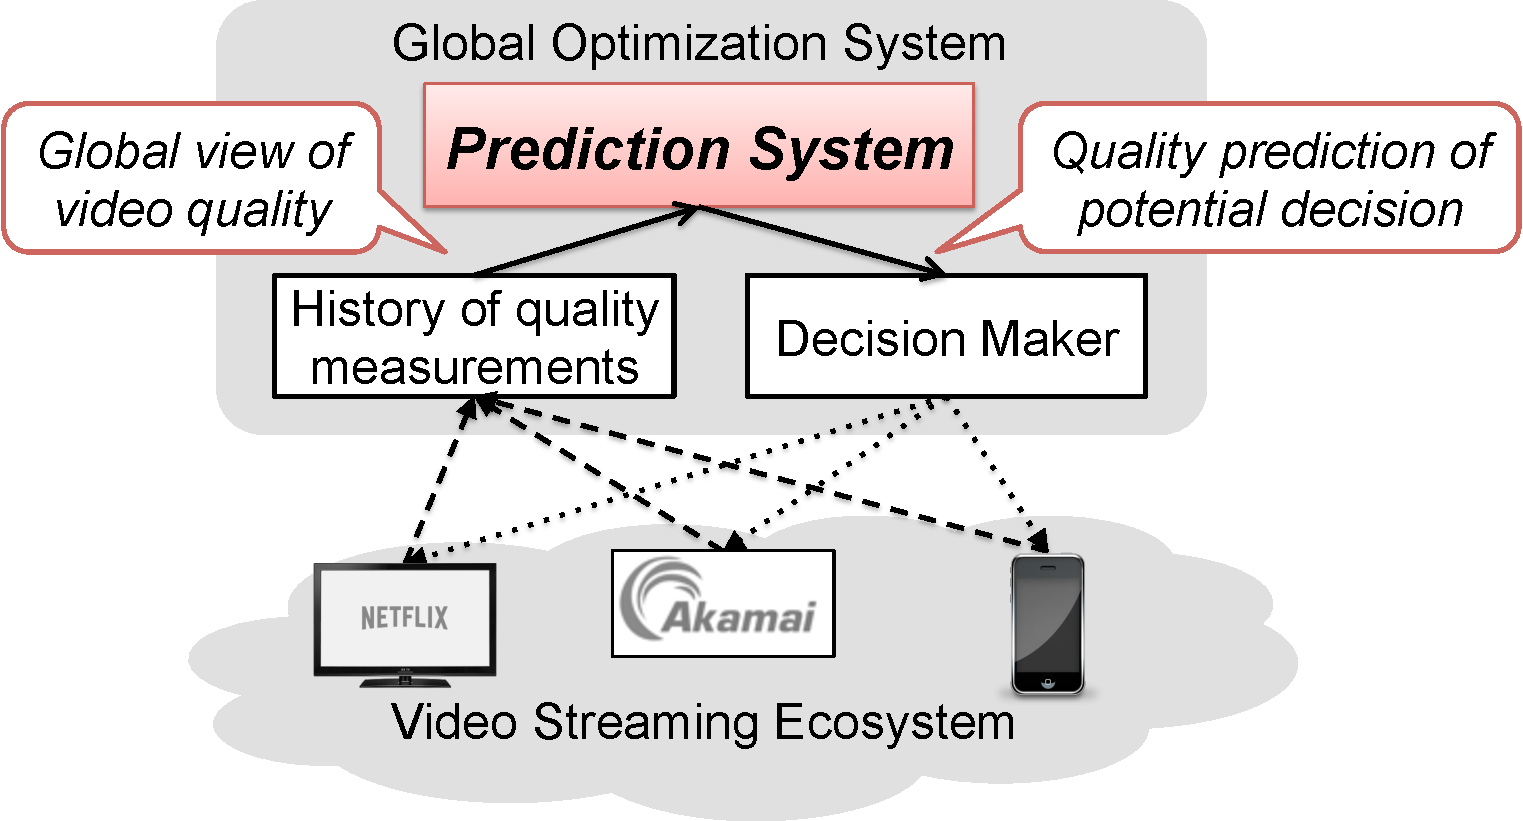
\includegraphics[width=.6\textwidth]{figures/cfa-controlplane-overview.pdf}
\caption{Overview of a \ControlPlane and the crucial role 
of a prediction system.}
\label{fig:globalsystem}
\end{figure}

In the context of video streaming, 
most video service providers today allow a 
video client (player) to switch CDN and bitrate 
among a set of available choices~\cite{sigcomm12,
c3,sigcomm12cdnmulti}.
%Today's video delivery systems allow each video client 
%(player) to switch CDN and bitrate among a set of 
%available choices. 
%\camera{Multi-CDN and multi-bitrate is commonly used by streaming video sites.}
These switches have little overhead and can be
performed at the beginning of and during a video 
playback~\cite{dash}. 
%\myparatight{Need for quality prediction}
Our goal then is to choose the best CDN and 
bitrate for a client by {\em accurately predicting 
the video quality of each hypothetical choice of 
CDN and bitrate}. 
In theory, if we can accurately predict the 
quality of each potential decision, then we 
can identify  the optimal decision.


To this end, we envision a prediction system that 
uses a {\em global view} of quality measurements to 
make predictions for a specific video session. % (i.e., pair of client and decision).
It learns a {\em prediction function} for each 
quality metric
$Pred:2^\HSessionFullSet\times\HSessionFullSet\mapsto \HReal$,
which takes as input a given set of historical 
sessions $\HSessionSet \in 2^\HSessionFullSet$ 
whose quality  is already measured, and a new 
session $\HSession\in\HSessionFullSet$, and 
outputs a quality prediction $p\in\HReal$ for 
$\HSession$.


%\myparatight{Quality metrics and session features} 
Each quality measurement %is a video session viewing a video 
summarizes the quality of a video session
for some duration of time (in our case, one minute). 
It is associated with values of four 
{\em quality metrics} (as defined in 
Section~\ref{subsec:related:video-qoe}) and 
a set of {\em features}
(summarized in Table~\ref{tab:features}).  
By feature,  we refer to the type of attribute 
(e.g., \fCDN), rather than value of these attributes 
(e.g., $\fCDN=Akamai$)
In general, the set of features depends on the degree 
of instrumentation and
what information is visible to a specific provider. 
For instance, a CDN may know the location of servers, 
whereas a third-party optimizer~\cite{conviva} may 
only have information at the CDN granularity. 
Our focus is not to determine the best set of 
features that should be recorded for each session, 
but rather engineer a prediction system that can 
take  an arbitrary set of features as inputs and 
extract the relationships between these features
and video quality. In practice, the above set of 
features can already provide accurate predictions 
that help improve quality.
% , and our approach can naturally include more
% features as they become available. 


\begin{table}[t!]
%\begin{footnotesize}
\begin{tabular}{p{3.8cm}|p{12cm}}
%{\bf Metrics} & {\bf Description} \\ \hline
%BufRatio & Fraction of time a session spends in buffering 
%(smooth playback is interrupted by buffering). \\ \hline
%AvgBitrate & Time-weighted average of bitrates in a session. \\ \hline
%JoinTime & Delay for the video to start playing from the 
%time the user clicks ``play''. \\ \hline
%Video start failure (VSF) & Fraction of sessions that fail to
% start playing (e.g., unavailable content or overloaded 
% server)\tablefootnote{For one session, VSF is zero if it 
% starts successfully, one otherwise.}. \\ \hline
{\bf Features} & {\bf Description} \\ \hline 
 \fASN &  Autonomous System to which client IP belongs. \\ \hline 
 \fCity &  City where the client is located.  \\ \hline
 \fConnectionType &  Type of access network; e.g.,  
 mobile/fixed wireless, DSL, fiber-to-home. \\ \hline
 \fPlayer & e.g.,  Flash, iOS, Silverlight,  HTML5. \\ \hline 
 \fSite & Content provider of requested video contents.\\ \hline%\tablefootnote{We use the terms site and content provider interchangeably.}. \\ \hline
 \fLiveOrVoD & Binary indicator of live vs.\ VoD content.\\ \hline 
 \fContentName & Name of the requested video object.\\ \hline 
 \fCDN &  CDN a  session started with. \\ \hline
 \fBitrate &  Bitrate value the session started at.
\end{tabular}
%\end{footnotesize}
\vspace{-0.2cm}
\caption{Quality metrics and session features associated 
with each session. 
\fCDN and \fBitrate refer to initial CDN/bitrate values as 
we focus on initial selections.}
\label{tab:features}
%\vspace{-0.5cm}
\end{table}

Our dataset consists of 6.6 million quality 
measurements collected from 2 million clients 
using 3 large public CDNs distributed across 
168 countries and 152 ISPs.

Next, we show real examples of the complex factors 
that impact video quality, and the limitations of strawman
solutions in capturing these relationships.

\subsection{Challenge 1: Complex QoE-Determining Factors}
\label{subsec:expressive}

\mypara{
High-dimensional relationship between video quality
and session features} 
Video quality could be impacted by {\em combinations} 
of multiple components in the network. 
Such high-dimensional effects make 
it harder to learn the relationships between video 
quality  and features, in contrast to simpler settings 
where features affect quality independently 
(e.g., assumed by Naive Bayes).
%quality prediction challenging since the 
%relationship between video quality and 
%features is more complex than if the impact of 
%individual features on quality is independent 
%(which is assumed by algorithms like Naive Bayes).




%\noindent\underline{Example of high dimensionality:}
%Here is an illustrative real-world example of high 
%dimensionality. 
In a real-world incident,
video sessions of Comcast users in Baltimore who watched 
videos from Level3 CDN experienced high failure rate (VSF) 
due to congested edge servers, shown by the blue line in 
Figure~\ref{fig:timeseries-expressive-model}.
The figure also shows the VSF of sessions sharing the same
values on one or two features with the affected sessions; 
e.g., all Comcast sessions across different cities and CDNs. 
In the figure, the high VSF of the affected sessions cannot be 
clearly identified if we look at the sessions 
 that match on only one or two features.
%does not suffice to clearly 
%none of the individual features or 
%two-feature combinations can clearly 
%show the high VSF of the affected sessions.
Only when three features of \fCDN (``Level3''), 
\fASN (``Comcast'') and \fCity (``Baltimore'') 
are specified (i.e., blue line), can we detect the 
high VSF and predict the quality of 
affected sessions accurately. 

\begin{figure}[t!]
\centering
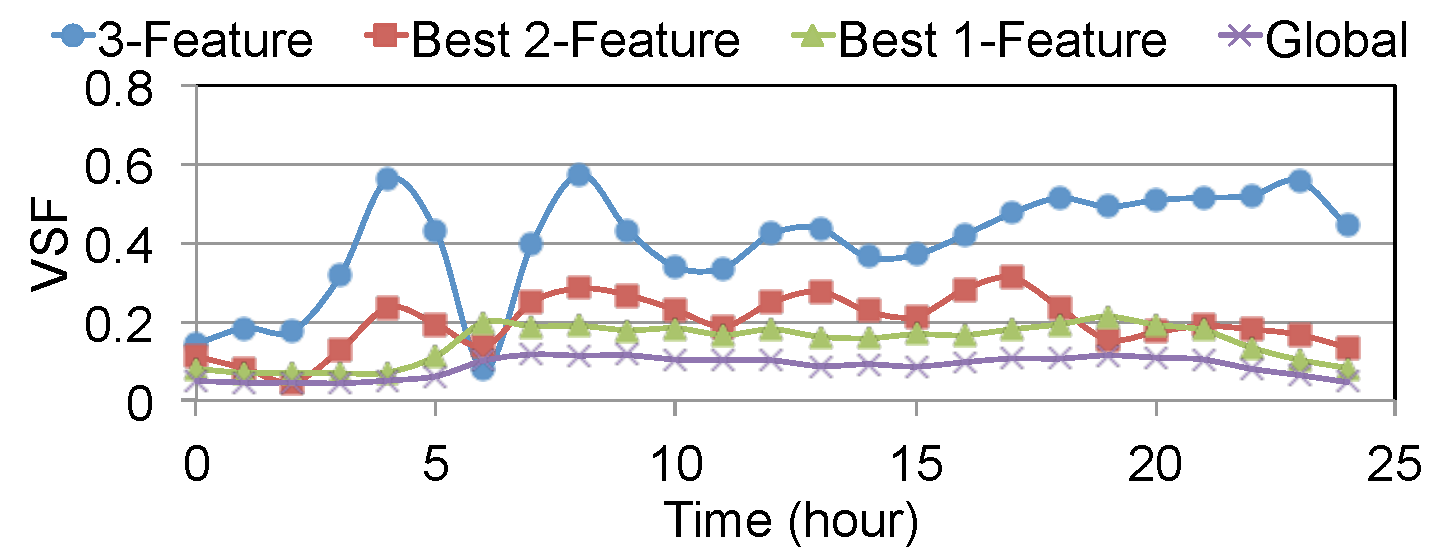
\includegraphics[width=0.65\textwidth]{figures/cfa-example-highdimension-timeseries.pdf}
\caption{The high VSF is only evident when three factors 
(CDN, ISP and geo-location) are combined.}
%\vspace{-0.2cm}
\label{fig:timeseries-expressive-model}
\end{figure}

 %One natural concern here is if this anecdotal evidence is an anomalous corner case.
% or if such high-dimensional 
%effects are  more pervasive. 
In practice, we find that such high-dimensional effects 
are the common case, rather than an anomalous corner case.  
For instance, more than 65\% of distinct
CDN-ISP-City values have VSF that is at least 50\% higher or 
lower than the VSF of sessions matching only one or 
two features (not shown). In other words, their quality is
affected by a combined effect of at least three features.

%\vyas{this doesnt address the concern. it  should have been across diff sessions/leaves :(}

\mypara{Limitation of existing solutions}
It might be tempting to develop  simple predictors; 
e.g., based on the last-hop 
connection by using average quality of history sessions 
with the same \fConnectionType value.
%\footnote{This is only an approximation to having the same last-hop capacity (we acknowledge that users of same connection type may have varying last-mile connection speed).}). 
However, they do not take into account the combined
impact of features on video quality.
Conventional machine learning techniques like Naive 
Bayes also suffer from the same limitation.
In Figures~\ref{subfig:quantitative-strawmen-lh} and 
\ref{subfig:quantitative-strawmen-nb},
we plot the actual JoinTime and the prediction
made by the last-hop predictor and Naive Bayes 
(from \texttt{Weka}~\cite{weka})
for 300 randomly sampled sessions.
The figures also show the mean relative error (
$\frac{|predicted-actual|}{actual}$).
For each session, the prediction algorithms train 
models using historical sessions within a 10-minute 
interval prior to the session under prediction.
It shows that the prediction error of both solutions is 
significant and two-sided (i.e., not fixable by
normalization).


\noindent{\bf Highly diverse structures of factors.}  
The factors that affect video quality vary across different sessions.
This means the prediction algorithm should be expressive enough
to predict quality for different sessions using 
different prediction models.
%\noindent\underline{Example of diversity:}
%Let us consider an illustrative example. 
%Many Flash video clients for whom Level3 
%edge servers provided high performance, and they had 
%good quality. 
%For these sessions, their quality is correlated with 
%a different set of features (\fCDN and \fPlayer) than 
%the example of high dimensionality (\fASN, \fCity and \fCDN).
For instance, the fact that many fiber-to-the-home (e.g., FiOS) 
users have high bitrates and people on 
 cellular connections have lower bitrates is largely due to 
the speed of their last-mile connection. In contrast, some video clients 
may experience video loading failures due to 
unavailability of specific content on some CDNs.
Chapter~\ref{ch:measurement}
has shown that many heterogeneous 
factors are correlated with video quality issues.
In Section~\ref{sec:cfa:outline}, we show  that 15\% of video 
sessions are impacted by more than 30 different combinations 
of features and give real examples of different factors that 
affect quality.

\noindent\underline{Limitation of existing solutions:}
To see why existing solutions are not sufficient, 
let us consider the $k$-nearest neighbor ($k$-NN) algorithm.
It does not handle diverse relationships between quality
and features, because the similarity between sessions
is based on the same function of features
independent of the specific session under prediction.
In Figure~\ref{subfig:quantitative-strawmen-nn},
we plot the actual values of JoinTime and the 
prediction made by $k$-NN with the same setup as 
Figure~\ref{subfig:quantitative-strawmen-lh}(b).
Similar to Naive Bayes and the last-hop predictor, 
$k$-NN has substantial prediction error.


\begin{figure}[t!]
\centering
\subfloat[Last hop (0.76)]
{
        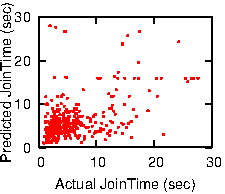
\includegraphics[width=0.3\textwidth]{figures/cfa-strawmen-scatter-comparison-naive.pdf}
        \label{subfig:quantitative-strawmen-lh}
}
\subfloat[Naive Bayes (0.61)]
{
        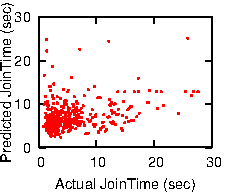
\includegraphics[width=0.3\textwidth]{figures/cfa-strawmen-scatter-comparison-2.pdf}
        \label{subfig:quantitative-strawmen-nb}
}
\subfloat[$k$-NN (0.63)]
{
        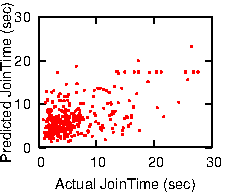
\includegraphics[width=0.3\textwidth]{figures/cfa-strawmen-scatter-comparison-1.pdf}
        \label{subfig:quantitative-strawmen-nn}
}
\caption{Prediction error of some existing solutions 
is substantial (mean of relative error in parentheses).}
%\vspace{-0.5cm}
\label{fig:quantitative-strawmen}
\end{figure}



\subsection{Challenge 2: Fresh Updates}
\label{subsec:fresh}

Video quality has significant temporal variability.
In Figure~\ref{fig:variability-all-metrics},
for each quality metric and combination of specific 
CDN, city and ASN, %(which reduces impact of the spatial variance), 
we compute the mean quality of sessions in each 
10-minute interval, and then plot the CDF of the 
relative standard deviation ($\frac{stddev}{mean}$)
%\footnote{Standard deviation divided by mean, which is used to normalize the scales of different quality metrics.} 
of the quality across different intervals.
In all four quality metrics of interest, we see 
significant temporal variability;
%on timescales of 10 minutes;
e.g., for 60\% of CDN-city-ASN combinations, 
the relative standard deviation of JoinTime across 
different 10-minute intervals is more than 30\%.
Such quality variability has also been confirmed in 
other studies (e.g.,~\cite{sigcomm12}).

The implication of such temporal variability
is that the prediction system must update models 
in near real-time.
In Figure~\ref{fig:strawman-staleness-all-metrics}, 
we use the same setup as 
Figure~\ref{fig:quantitative-strawmen}, except that the 
time window used to train prediction models is 
several minutes prior to the session under prediction.
The figure shows the impact of such staleness on 
the prediction error for JoinTime. 
For both algorithms, prediction error increases 
dramatically if the staleness exceeds 10 minutes. 
As we will see later, this negative impact of staleness 
on accuracy is not specific to these prediction 
algorithms (Section\ref{subsec:eval-scalability}). 
%This means the prediction system must update models  
%in near real-time.



\mypara{Limitation of existing solutions}
The requirement to use the most recent measurements
makes it infeasible to use computationally expensive models.
%models, such Support Vector Machines (SVM).
For instance, it takes at least one 
hour to train an SVM-based prediction model from 15K
quality measurements in a 10-minute interval for 
one video site, so the quality predictions 
will be based on information from more than one hour ago.


\begin{figure}[t!]
\centering
\subfloat[Temporal variability]
{
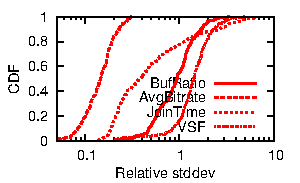
\includegraphics[width=.45\textwidth]{figures/cfa-stddev-metrics.pdf}
        \label{fig:variability-all-metrics}
}
\subfloat[Impact of staleness on accuracy]
{
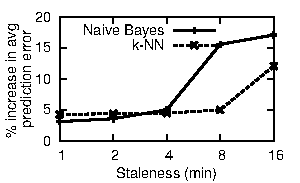
\includegraphics[width=.45\textwidth]{figures/cfa-strawman-staleness.pdf}
        \label{fig:strawman-staleness-all-metrics}
}
\caption{Due to significant temporal variability of video quality (left), 
prediction error increases dramatically with stale data (right).}
%\vspace{-0.2cm}
\label{fig:temporal-variability}
\end{figure}


%In summary, the ideal predictor should (a) capture the 
%complex relationship between features and video 
%quality, and (b) predict quality based on fresh data. 

%We will present \dda to achieve these goals in the
%next sections.

%{
%\begin{table}[h!]
%%\begin{small}
%\begin{tabular}{p{6cm}|p{3.5cm}|p{3cm}}
%   &\textbf{Expressive models} & \textbf{Fresh updates} \\ \hline
%Naive models (e.g., last-mile)                       & $\times$          & $\checkmark$         \\ \hline
%Simple ML (e.g., NB, k-NN)                       & $\times$          & $\checkmark$         \\ \hline
%Complex ML (e.g., SVM)	                            & ?                 & $\times$             \\ \hline 
%{\bf The ideal (CFA)}                                 & {\bf $\checkmark$} & {\bf $\checkmark$}
%\end{tabular}
%%\end{small}
%%\vspace{-0.3cm}
%\caption{Analysis of existing solutions in the lense of the two challenges.}
%%\vspace{-0.2cm}
%\label{tab:qualitative-strawmen}
%\end{table}
%}














\section{Overview of CFA Ideas}
\label{sec:cfa:outline}


This section presents the domain-specific insights we use to 
help address the expressiveness challenge 
(Section~\ref{subsec:expressive}).  
The first insight is that sessions matching on all features 
have similar video quality.  
However, this approach suffers from the curse of dimensionality.
%it is challenging to translate this insight into an actionable approach because
%it suffers from the classical curse of dimensionality -- hard to find
%a sufficient number of identical sessions.  
Fortunately,  we can leverage a second insight that 
each video session has a subset of {\em critical features} 
that ultimately determine its video quality. 
 % and we can use  it to tackle the curse of dimensionality. 
We conclude this section  by highlighting two outstanding 
issues in translating these insights into  a practical 
prediction system.



\subsection{Baseline Prediction Algorithm}
\label{subsec:cfa:outline:basic}

Our  first insight is that 
%there is some inherent
%network/application structure because of which 
sessions that have identical  feature values will 
naturally have similar (if not identical) quality. 
 For instance, we expect that all Verizon 
 FiOS users  viewing a specific  HBO  video 
using Level3 CDN in Pittsburgh at Fri 9 am should 
have similar quality (modulo very user-specific  effects 
such as local Wi-Fi interference inside the home).
We can summarize the intuition as follows:

\begin{insight}
\vspace{0.1cm}
At a given time, video sessions having same value 
on every feature have similar video quality.
\vspace{-0.2cm}
\label{insight:1}
\end{insight}


%\camera{\insightref{insight:1} is merely a motivation.}
Inspired by \insightref{insight:1}, we can consider a 
baseline algorithm (Algorithm~\ref{alg:baseline}).
We predict a session's quality based on ``identical
sessions'', i.e., those from recent history that match 
values on {\em all} features with the session under 
prediction. 
Ideally, given infinite data, this 
%simple domain-specific engineered 
algorithm is accurate, because it can capture
all possible combinations of factors affecting 
video quality.


\begin{algorithm}[t!]
\begin{small}
 \KwIn{Session under prediction \HSession, Previous sessions \HSessionSet}
 \KwOut{Predicted quality $p$}
 \tcc{\footnotesize{$S'$:identical sessions matching on all features with \HSession in recent history(\HTimeWindowEst)}}
 $S'\leftarrow\HSimilarSessionSet{\HSession}{\HSessionSet}{AllFeatures}{\HTimeWindowEst}$\;
 \tcc{\footnotesize{Summarize the quality (e.g.,median) of the identical sessions in $S'$.}}
 $p\leftarrow\HEst{S'}$\;
 \Return{$p$}\;
\end{small}
 \caption{{\bf {\em Baseline prediction that finds sessions matching on all features and uses their 
 observed quality as the basis for prediction.  %Unfortunately, it suffers from the curse of dimensionality.
 }}}
\label{alg:baseline}
\end{algorithm}

 

%\begin{figure}[h!]
%\centering
%\includegraphics[width=0.4\textwidth]{eval-figs/batch-3/neighbor-count.pdf}
%\vspace{-0.1cm}
%\tightcaption{More than 90\% of sessions have at most one identical session within 5-min window.}
%\vspace{-0.1cm}
%\label{fig:infeasible-nn}
%\end{figure}

However, this algorithm is unreliable as it suffers from the 
classical curse of 
dimensionality~\cite{powell2007approximate}. 
Specifically, given the number of combinations 
of feature values (ASN, device, content providers, 
CDN, just to name a few), it is hard to find enough identical 
sessions needed to make a robust prediction. 
In our dataset, more than 78\% of sessions have no 
identical session (i.e., matching on all features)
within the last 5 minutes.
%more than 78\% of sessions within a 5-minute time window
%have no identical session (i.e., matching on all features).
%Thus, we do not have sufficient data to make reliable predictions.


\subsection{Critical Features}
\label{subsec:cfa:outline:critical}

 In practice, we expect that some features are
more likely to  ``explain'' the observed quality 
of a specific video session than others.  
For instance, if a specific peering point
between Comcast and Netflix in New York is 
congested, then we expect most of these users 
will suffer poor quality, regardless of the speed of 
their local connection. 
%Similarly, we can roughly expect most 
% fiber-to-the-home (e.g., FiOS) users to have high bitrates and people on 
% cellular connections to have lower bitrates. We can formalize this as follows:

\begin{insight}
\vspace{0.1cm}
Each video session has a subset of {\em critical features} that ultimately determines its video quality.
\vspace{-0.2cm}
\end{insight}

We already saw some real examples in 
Section~\ref{subsec:expressive}:
%To see some real-world examples of critical features, we 
%consider two examples in \Section\ref{subsec:expressive}.
in the example of high dimensionality, the critical features 
of the sessions affected by the congested Level3 edge 
servers are $\{\fASN, \fCDN, \fCity\}$;
in the examples of diversity, the critical features are
$\{\fConnectionType\}$ and $\{\fCDN,\fContentName\}$.
Table~\ref{tab:bottleneck} gives more real examples 
of critical features that we have observed in operational 
settings and confirmed with domain experts.


\begin{table}[t!]
%\begin{small}
    \begin{tabular}{p{2.in}|p{2in}}
    {\bf Quality issue} & {\bf Set of critical features} \\ \hline\hline
%    Software update on OS & \{OS\}  \\ \hline
%    Player bitrate-adaptation logic & \{PlayerName\}  \\ \hline
%    Device  on cellular signal  & \{Device,ConnectionType\}  \\ \hline
%    Load of CDN1 server in city  & \{CDN,City\}      \\ \hline
%    Link congestion between CDN1 server in city and ASN    & \{CDN,City,ASN\}    \\ \hline
%    Bad Live feeds from one site to CDN1  & \{Site,LiveOrVod,CDN\} \\

     Issue on one player of Vevo & $\{\fPlayer,\fSite\}$ \\ \hline
     ESPN flipping between CDNs  & $\{\fCDN,\fSite,\fContentName\}$ \\ \hline
     Bad Level3 servers for Comcast users in Maryland& $\{\fCDN,\fCity,\fASN\}$ \\
    \end{tabular}
\caption{Real-world examples of critical features confirmed 
by analysts at a large video optimization vendor.}
\label{tab:bottleneck}
%\end{small}
%\vspace{-0.2cm}
\end{table}


A natural implication of this insight is that it can help us 
tackle  the curse of dimensionality.
Unlike Algorithm~\ref{alg:baseline}, which fails to find a 
sufficient number of sessions,
%Instead of failing to find a sufficient number of identical sessions that match on all 
%features (Algorithm~\ref{alg:baseline}), 
we can estimate quality more reliably by aggregating 
observations across a larger amount of ``similar sessions'' that 
only need to match on these {\em critical features}. 
Thus, critical features can provide expressiveness
while avoiding curse of dimensionality.

Algorithm~\ref{alg:critical-feature} presents a logical 
view of this idea:
%We use two logical steps to predict quality of session  $\HSession$.
\begin{packedenumerate}
\item {\bf Critical feature learning (line 1):} 
First, find the critical features of each session $\HSession$, 
denoted as $\HCriticalFeature{\HSession}$.
\item {\bf Quality estimation (line 2, 3):}
Then, find similar sessions that match values with 
$\HSession$ on critical features 
$\HCriticalFeature{\HSession}$ 
within a recent history of length $\HTimeWindowEst$ 
(by default, 5 minutes). 
Finally, return some suitable estimate of the quality of 
these similar sessions; 
e.g., the median\footnote{We use median because it 
is more robust to outliers.} 
(for BufRatio, AvgBitrate, JoinTime) or the mean (for VSF).
\end{packedenumerate}



\begin{algorithm}[t!]
\begin{small}
 \KwIn{Session under prediction \HSession, Previous sessions \HSessionSet}
 \KwOut{Predicted quality $p$}
 \tcc{\footnotesize{$CF_{\HSession}$:Set of critical features of \HSession}}
 $CF_{\HSession}\leftarrow\HCriticalFeature{\HSession}$\;
 \tcc{\footnotesize{$S'$:Similar sessions matching values on 
critical features $CF_{\HSession}$ with \HSession.}}
 $S'\leftarrow\HSimilarSessionSet{\HSession}{\HSessionSet}{CF_{\HSession}}{\HTimeWindowEst}$\;
 \tcc{\footnotesize{Summarize the quality of the similar sessions in $S'$.}}
 $p\leftarrow\HEst{S'}$\;
 \Return{$p$}\;
\end{small}
 \caption{{\bf {\em \dda prediction algorithm, where prediction is based on 
similar sessions matching on critical features.}}}
\label{alg:critical-feature}
\end{algorithm}



A practical benefit of Algorithm~\ref{alg:critical-feature} 
is that it is interpretable~\cite{vellido2012making}, 
unlike some machine learning algorithms (e.g., PCA or SVM).
%quality predictions are interpretable.
This allows domain experts to combine their knowledge 
with \dda
%(e.g., directly setting critical features of sessions) 
and diagnose prediction errors or resolve incidents, 
as we explore in Section~\ref{subsec:insight-value}. 

At this time, it is useful to clarify what critical features 
are and what they are not.
In essence, critical features provide the explanatory 
power of how a prediction is made.
However, critical features are not a minimal set of 
factors that determine the quality (i.e., root cause). 
That is, they can include both features that reflect 
the root cause as well as additional features.
For example, if all HBO sessions use Level3, their 
critical features may include both \fCDN and \fSite, 
even if \fCDN is redundant, since including it does 
not alter predictions. 
The primary objective of \dda is accurate prediction; 
root cause diagnosis may be an added benefit.







\section{Design of CFA}
\label{sec:cfa:design}

In this section, we present the detailed design of \dda 
and discuss how we address the two practical challenges 
mentioned in the previous section: learning critical features 
and reducing update delay.

The key  to addressing these challenges
%,  which leads 
% to the practical realization of \dda, 
 is our third and final domain-specific insight:

\begin{insight}
\vspace{0.1cm}
Critical features tend to {\em persist} on long timescales
of tens of minutes.
\vspace{-0.2cm}
\label{insight:persistence}
\end{insight}

 This insight is derived from prior measurement 
 studies.
 For instance, our measurement study in 
 Chapter~\ref{ch:measurement} 
 on shedding light on video quality issues in the wild showed 
 that the factors that lead to poor video quality persist
 for hours, and sometimes even days.  
 Another recent study from the C3 system suggests that 
 the best CDN tends to be relatively stable on the 
 timescales of few tens of minutes~\cite{c3}.  
We independently confirm this observation in 
Section~\ref{subsec:eval-scalability} that 
using slightly stale critical features (e.g., 30-60 minutes 
 ago) achieves similar prediction accuracy as using the 
most up-to-date critical features.
Though this insight holds for most cases, it is still possible
(e.g., on mobile devices) that critical features persist on a 
relatively shorter timescale (e.g., due to the nature of 
mobility).
%For instance, on a mobile device, the persistency of critical features
%might be shorter than tens of minutes due to the nature of mobility.}


% we show that using slightly stale 
%^critical features (i.e., learned 30-60 minutes ago) achieves
%s%imilar prediction accuracy as using the most up-to-date 
%c%ritical features, suggesting that the persistence of critical 
%features is on timescale of tens of minutes.

Note that the persistence of critical features does not 
mean that quality values are equally persistent.  
In fact, persistence of critical features is on a 
timescale an order of magnitude longer than 
the persistence of quality.  
That is, even if quality fluctuates rapidly, the critical 
features that determine the quality do not change 
as often.


As we will see below, this persistence enables 
(a) automatic learning  of critical features from history, 
and (b) a scalable workflow that provides 
up-to-date estimates. 


\subsection{Learning Critical Features}
\label{subsec:cfa:design:learning}

Recall that the first challenge is
% that we cannot statically map each
%session to its critical features 
obtaining the critical features for each session.
The  persistence of  critical features has a natural 
corollary that we can use to automatically learn them: 

\begin{imp}
\vspace{0.1cm}
Persistence  implies that 
critical features of a session are learnable from history.
\vspace{-0.6cm}
\label{imp:learning}
\end{imp}

%The key notation is {\em \HSimSessSet}
%$\HSimilarSessionSet{\HSession}{\HSessionSet}{\HFeatureSet}{\HTimeWindow}$, which consists of sessions in $\HSessionSet$ that match $\HSession$ on features in $\HFeatureSet$ and happened within time window $\HTimeWindow$ before $\HSession$. 
%For instance, $\HSimilarSessionSet{\HSession}{\HSessionSet}{\{CDN\}}{\textrm{5 minutes}}$ 
%includes all sessions that use same CDN with $\HSession$ 
%and happened within 5 minutes before $\HSession$. 
%Note that, prediction made by Algorithm~\ref{alg:critical-feature} is 
%$\HPred{\HSession}{\HSessionSet}=\HEst{\HSimilarSessionSet{\HSession}{\HCriticalFeature{\HSession}}{\HFeatureSet}{\HTimeWindow}}$.


\begin{table}[t!]
%\begin{footnotesize}
\begin{tabular}{p{3.5cm}|p{3cm}|p{7.5cm}}
{\bf Notations} & {\bf Domains} & {\bf Definition} \\ \hline\hline
$\HSession,\HSessionSet,\HSessionFullSet$ & & A session, a set of sessions, set of all sessions \\ \hline
%$\HSession$ & & A video session \\ \hline
%$\HSessionSet$ & & A set of video sessions \\ \hline
%$\HSessionFullSet$ & & Set of all video sessions \\ \hline
%$\HSessionTime{\HSession}$ & $\HSessionFullSet\mapsto\HReal$ & Timestamp of $\HSession$ \\ \hline
$\HSessionQuality{\HSession}$ & $\HSessionFullSet\mapsto\HReal$ & Quality of $\HSession$ \\ \hline
$\HDistribution{\HSessionSet}$ & $2^\HSessionFullSet\mapsto2^\HReal$ & $\{\HSessionQuality{\HSession}|\HSession\in\HSessionSet\}$ \\ \hline
%$\HEst{\HSessionSet}$ & $2^\HSessionFullSet\mapsto\HReal$ & Summarizing value (by default, median) of $\HDistribution{\HSessionSet}$ \\ \hline
%$\HDist{\HSessionSet_1}{\HSessionSet_2}$ & $2^\HSessionFullSet\times2^\HSessionFullSet\times\HReal$ & JS divergence of $\HDistribution{\HSessionSet_1}$ and $\HDistribution{\HSessionSet_2}$\\ \hline
$\HFeature,\HFeatureSet,\HFeatureFullSet$ & & A feature, a set of features, set of all features \\ \hline
%$\HFeature$ & & A session feature \\ \hline
%$\HFeatureSet$ & & A set of session features \\ \hline
%$\HFeatureFullSet$ & & Set of all session features \\ \hline
$\HCriticalFeature{\HSession}$ & $\HSessionFullSet\mapsto2^\HFeatureFullSet$ & Critical features of $\HSession$ \\ \hline
$\HFeatureValueFullSet$ & & Set of all feature values \\ \hline
$\HFeatureValue{\HFeature}{\HSession}$ & $\HFeatureFullSet\times\HSessionFullSet\mapsto\HFeatureValueFullSet$ & Value on feature $\HFeature$ of $\HSession$ \\ \hline
$\HFeatureSetValue{\HFeatureSet}{\HSession}$ & $2^\HFeatureFullSet\times\HSessionFullSet\mapsto2^\HFeatureValueFullSet$ & Set of values on features in $\HFeatureSet$ of $\HSession$ \\ \hline
$SimilarSessionSet$ $(\HSession,\HSessionSet,\HFeatureSet,\HTimeWindow)$ & $\HFeatureFullSet\times2^\HFeatureFullSet\times\HSessionFullSet\times\HReal^{+}\mapsto2^\HFeatureFullSet$ & $\{\HSession'|\HSession'\in\HSessionSet,\HSessionTime{\HSession}-\HTimeWindow<\HSessionTime{\HSession'}<\HSessionTime{\HSession},\HFeatureSetValue{\HFeatureSet}{\HSession'}=\HFeatureSetValue{\HFeatureSet}{\HSession}\}$ \\ 
%\hline
%$\HPred{\HSession}{\HSessionSet}$ & $\HSessionFullSet\times2^\HSessionFullSet\mapsto\HReal$ & Prediction function
\end{tabular}
%\end{footnotesize}
\caption{Notations used in learning of critical features.}
\label{tab:terminology}
%\vspace{-0.5cm}
\end{table}



Specifically, we can simply look back over the history and identify  
the subset of features $\HFeatureSet$ such that the quality 
distribution of sessions matching on $\HFeatureSet$ is most similar 
to that of sessions matching on {\em all} features.   
For instance, suppose we have three features
$\langle \mathit{ContentName},\mathit{ASN},\mathit{CDN}\rangle$ and 
it turns out that sessions with  $\mathit{ASN}=\mathit{Comcast},
\mathit{CDN}=\mathit{Level3}$ consistently
have  high buffering over the last few hours due to some internal 
congestion at the corresponding exchange point. 
Then, if we look back over the last few hours, the data from 
history will   naturally reveal  that the distribution of the quality of 
sessions  with the feature values
$\langle\mathit{ContentName}=\mathit{Foo},
\mathit{ASN}=\mathit{Comcast},\mathit{CDN}=\mathit{Level3}\rangle$
will be  similar to $\langle \mathit{ContentName}=\mathit{*},
\mathit{ASN}=\mathit{Comcast},\mathit{CDN}=\mathit{Level3} \rangle$, 
but very different from, say, the quality of sessions in 
$\langle \mathit{ContentName}=\mathit{*},\mathit{ASN}=\mathit{*},
\mathit{CDN}=\mathit{Level3} \rangle$,
or $\langle \mathit{ContentName}=\mathit{*},
\mathit{ASN}=\mathit{Comcast},\mathit{CDN}=\mathit{*} \rangle$.
Thus, we can use a data-driven approach to learn that 
$\mathit{ASN},\mathit{CDN}$ are the critical features for sessions 
matching $\langle \mathit{ContentName}=\mathit{Foo},
\mathit{ASN}=\mathit{Comcast},\mathit{CDN}=\mathit{Level3} \rangle$.




% irrespective  of other feature values, sessions wit history that predicting the quality 
  



%Inspired by \impref{imp:learning}, we learn critical features 
%over a time window, during which critical features persist. 
%Intuitively, critical features are the subset of features 
%that meet two requirements.
%\begin{packeditemize}
%\item First, there should enough sessions
%for quality estimation of Algorithm~\ref{alg:critical-feature}
%to avoid unreliable prediction due to curse of dimensionlity.
%This is guaranteed by line 7-9.
%\item Second, among subsets of features that meet the first 
%requirement, we find the subset of features $\HFeatureSet$ such that 
%quality distribution of sessions matching $\HFeatureSet$ is the 
%most similar to that of sessions matching all features
%, 
%because these two sets of sessions should be determined by 
%the same set of critical features.
%\end{packeditemize}
%Finally, we should take into account two key aspects of model 
%expressiveness (\Section\ref{subsec:expressive}):
%high diversity (critical features are learned for each session 
%under prediction), and high dimensionality (critical features could be 
%any subsets of features). 


\begin{algorithm}[t!]
\begin{small}
 \KwIn{Session under prediction \HSession, Previous sessions \HSessionSet}
 \KwOut{Critical features for  \HSession}
 \tcc{Initialization}
 $\mathit{MaxSimilarity}\leftarrow-\infty,\mathit{CriticalFeatures}\leftarrow \mathit{NULL}$\;
 %\tcc{$D_{finest}$:Quality distribution of \HSimilarSessionSet{\HSession}{\HSessionSet}{\HFeatureFullSet}{\HTimeWindowLearn}.}
 \tcc{$D_{finest}$:Quality distribution of sessions matching on $\HFeatureFullSet$ in $\HTimeWindowLearn$.}
 $D_{finest}\leftarrow\HDistribution{\HSimilarSessionSet{\HSession}{\HSessionSet}{\HFeatureFullSet}{\HTimeWindowLearn}}$\;
 \For{$\HFeatureSet\subseteq2^\HFeatureFullSet$}{
	\tcc{Exclude $\HFeatureSet$ without enough similar sessions for prediction.}
	\If{$|\HSimilarSessionSet{\HSession}{\HSessionSet}{\HFeatureSet}{\HTimeWindowEst}|<n$}{{\bf continue\;}}
 	%\tcc{$D_{\HFeatureSet}$:Quality distribution of \HSimilarSessionSet{\HSession}{\HSessionSet}{\HFeatureSet}{\HTimeWindowLearn}.}
	\tcc{$D_{\HFeatureSet}$:Quality distribution of sessions matching on $\HFeatureSet$ in $\HTimeWindowLearn$.}
	$D_{\HFeatureSet}\leftarrow\HDistribution{\HSimilarSessionSet{\HSession}{\HSessionSet}{\HFeatureSet}{\HTimeWindowLearn}}$\;
	\tcc{Get similarity of $D_{finest}$ \& $D_{\HFeatureSet}$.}
	$\mathit{Similarity}\leftarrow\HDist{D_{\HFeatureSet}}{D_{finest}}$\; 	\If{$\mathit{Similarity}>\mathit{MaxSimilarity}$}{
		$\mathit{MaxSimilarity}\leftarrow \mathit{Similarity}$\;
		$\mathit{CriticalFeatures}\leftarrow \HFeatureSet$\;
	}
 }
 \Return{CriticalFeature}\;
\end{small}
 \caption{{\bf {\em Learning of critical features.}}}
\label{alg:learning}
\end{algorithm}

Algorithm~\ref{alg:learning}  formalizes this intuition for learning 
critical features. 
Table~\ref{tab:terminology} summarizes the notation used in
Algorithm~\ref{alg:learning}.
For each subset of features $\HFeatureSet$ (line 3), 
we compute the similarity between the quality distribution 
($D_{\HFeatureSet}$) of sessions matching on $\HFeatureSet$ 
and the quality distribution ($D_{finest}$) of sessions
matching on all features (line 7). 
% \vyas{please refer to the pseudocode in the text with the line numbers etc. dont just 
%assume ppl will read pseudocode and follow!!}
Then, we find the $\HFeatureSet$ that yields the maximum 
similarity (line 8-10), under one additional constraint that 
$\HSimilarSessionSet{\HSession}{\HSessionSet}{\HFeatureSet}{\HTimeWindowEst}$ 
should include enough (by default, at least 10) sessions to get 
reliable quality estimation (line 4-5).
%there
%should be enough sessions to  get reliable quality
%estimates, i.e., $\HSimilarSessionSet{\HSession}{\HSessionSet}{\HFeatureSet}{\HTimeWindowEst}$
%needs to have at least $n$ (by default, 10) sessions (line 4-5).
This check ensures that the algorithm will not simply return the set of all features.



As an approximation of the duration in which critical features 
persist, we use $\HTimeWindowLearn=60min$.
Note that $\HTimeWindowLearn$ is an order of magnitude 
larger than the time window $\HTimeWindowEst$ used in 
quality estimation, because critical features persist on a 
much longer timescale than quality values.
%Default value of $n$ is 10 sessions. 
We use (the negative of) Jensen-Shannon 
divergence between $D_1$ and $D_2$ to quantify their 
similarity $\HDist{D_1}{D_2}$.
%(assuming both of them are draw from a normal distribution).





Although Algorithm~\ref{alg:learning} can handle most cases, 
there are corner cases where
$\HSimilarSessionSet{\HSession}{\HSessionSet}
{\HFeatureFullSet}{\HTimeWindowLearn}$ 
does not have enough sessions (i.e., more than $n$) to 
%learn $\HCriticalFeature{\HSession}$ reliably. 
compute $\HDist{D_{\HFeatureSet}}{D_{finest}}$ reliably. 
In these cases, we replace $D_{finest}$ by the set of $n$ 
sessions that share most features with $\HSession$ 
over the time window of $\HTimeWindowLearn$. 
Formally, we use 
$\{\HSession'|\HSession'\textrm{ matches $k_{\HSession}$ 
features with }\HSession\}$, 
where $k_{\HSession}=\argmin_k\left(|\{\HSession'|\HSession'\textrm{ matches $k$ features with }\HSession\right|\geq n\}|)$.





\subsection{Using Fresh Updates}
\label{subsec:scalability}

Next, we focus on reducing the update delay
between when a quality measurement is received and 
used for prediction. 



Naively running critical feature learning and quality 
estimation of Algorithm~\ref{alg:critical-feature}
can be time-consuming, causing the predictions to 
rely on stale data.
In Figure~\ref{fig:scalable-workflow}(a), $T_{CFL}$ and 
$T_{QE}$ are the duration of critical feature learning and 
the duration of quality estimation, respectively. 
The staleness of quality estimation (depicted in 
Figure~\ref{fig:scalable-workflow}) 
to respond to a prediction query can be as large as the 
total time of two steps (i.e., $T_{CFL}+T_{QE}$), which 
typically is tens of minutes 
(Section~\ref{subsec:eval-scalability}).
%This is because the critical feature learning (line 1) typically takes tens of 
%minutes to update its results (\Section\ref{subsec:eval-scalability}).
%To see why, consider Figure~\ref{fig:scalable-workflow}(a), where $T_{CFL}$ and $T_{QE}$ are the duration
%of critical feature learning and the duration of quality estimation, respectively. 
%To respond a prediction query, the staleness of quality estimation is up to the total time 
%of two steps (i.e., $T_{CFL}+T_{QE}$).
Also, simply using more parallel resources is not sufficient. 
The time to learn critical features using
Algorithm~\ref{alg:learning} grows linearly with the number of 
sessions under prediction, the number of history sessions,
and the number of possible feature combinations.
Thus, the complexity of learning critical features $T_{CFL}$ is 
exponential in the number of features. Given the current 
set of features, $T_{CFL}$ is on the scale of tens of minutes.

%This means the complexity of learning critical features is 
%super-linear to the size of data (number of sessions and 
%number of available features). Thus, simply adding more 
%resources will not suffice.

\begin{figure}[t!]
\centering
%\vspace{-0.3cm}
%\hspace{-0.6cm}
%\subfigure[Naive workflow]
%{
%\includegraphics[width=0.25\textwidth]{figures/scalability-naive.pdf}
%\label{subfig:scalability-naive}
%}
%\hspace{-0.4cm}
%\subfigure[CFA workflow]
%{
%\includegraphics[width=0.25\textwidth]{figures/scalability-cfa.pdf}
%\label{subfig:scalability-cfa}
%}
%\hspace{-0.6cm}
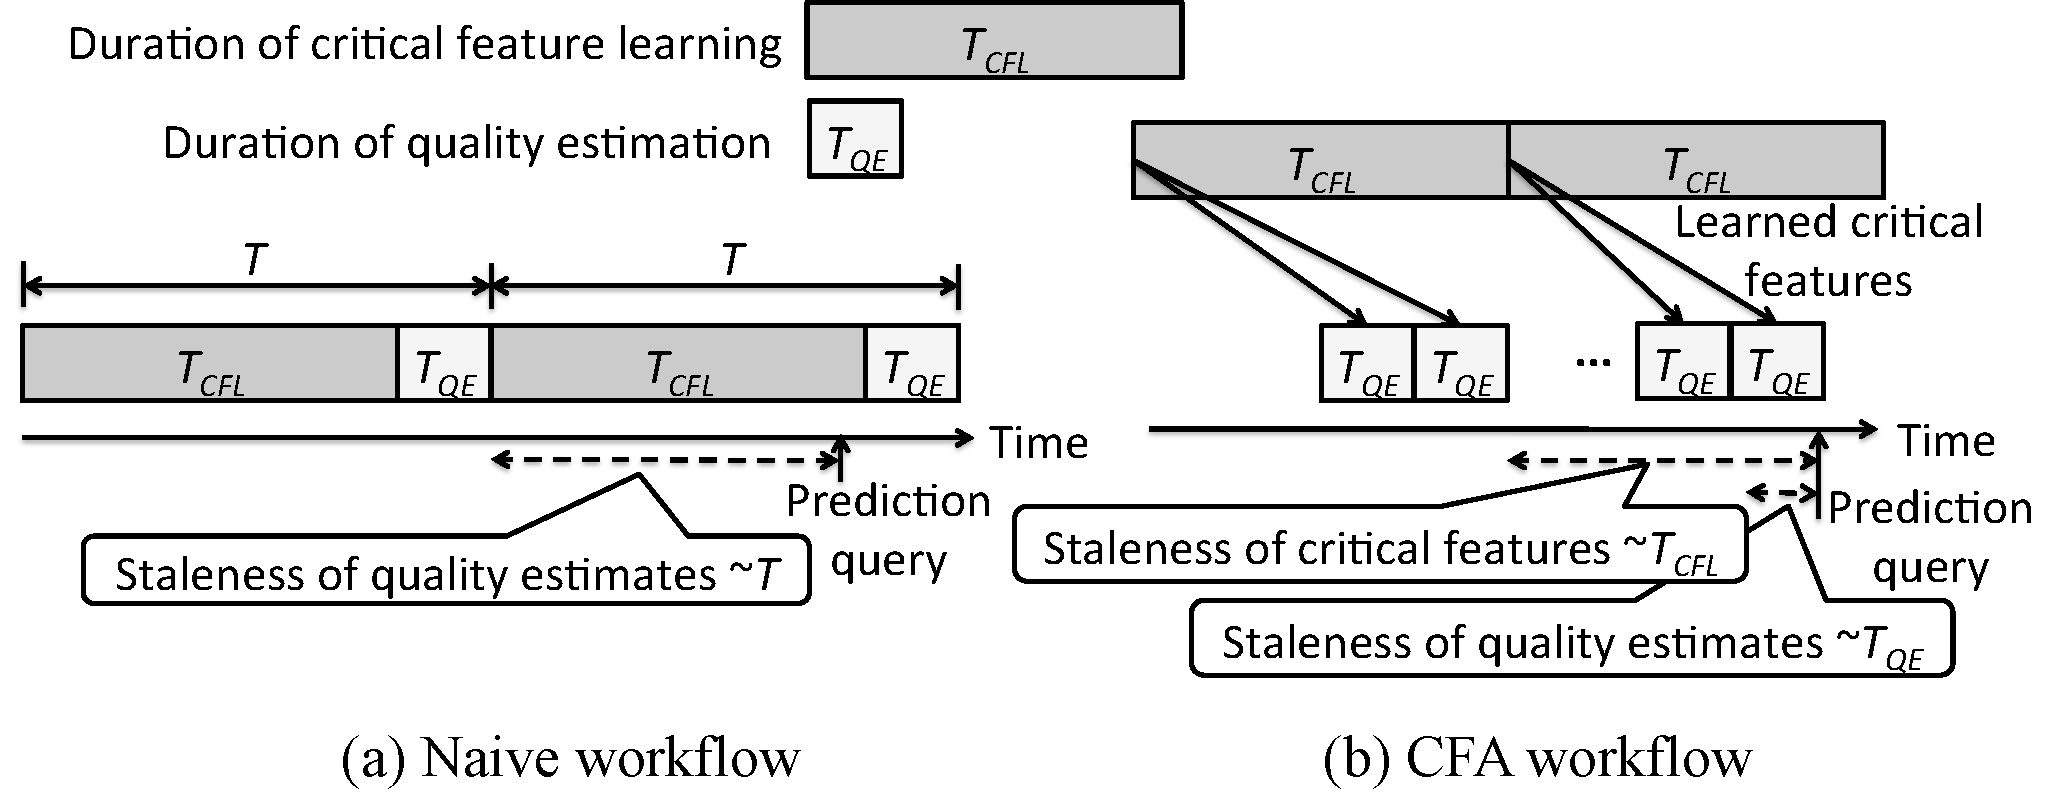
\includegraphics[width=0.85\textwidth]{figures/cfa-scalability-naive-cfa.pdf}
\caption{To reduce update delay, we run critical feature learning 
and quality estimation at different timescales by leveraging 
persistence of critical features.}
\label{fig:scalable-workflow}
\end{figure}

To reduce update delay, we again leverage the 
persistence of critical features:

\begin{imp}
\vspace{0.1cm}
Persistence implies that critical features can be cached and reused
 over tens of minutes.
 \vspace{-0.3cm}
\label{imp:reducing}
\end{imp}


 Building on \impref{imp:reducing}, we decouple the 
critical feature learning and quality estimation steps, and run
them at separate timescales.
On the timescale of tens of minutes, we update the results of 
critical feature learning. Then, on a faster timescale of tens of seconds, 
we update quality estimation using fresh data and the most recently
learned critical features. 

This decoupling 
%ensures that each step 
%can update its result sufficiently frequently to 
minimizes the impact of staleness on prediction accuracy.
Learning critical features on the timescale of tens 
of minutes
%\camera{\footnote{Learning critical features on a much larger set of features could take longer, 
%but it is enough for the current set of features, and the feature set will not grow very quickly.}}
is sufficiently fast as they persist 
on the same timescale.
%Since critical features persist, learning them
%on the timescale of tens of minutes is sufficient to capture their dynamics.
Meanwhile, %based on learned critical features, 
quality estimation can be updated every tens of seconds 
and makes predictions based on quality updates with sufficiently
low staleness.
Thus, the staleness of quality estimation $T_{QE}$ of
the decoupled workflow (Figure~\ref{fig:scalable-workflow}(b))
is a magnitude lower than $T_{QE}+T_{CFL}$ of the naive workflow 
(Figure~\ref{fig:scalable-workflow}(a)).
In Section~\ref{subsec:eval-scalability}, we show that 
this workflow can retain the freshness of critical features and quality estimates.
%\camera{It should be noticed that, though $T_{QE}+T_{CFL}$ (tens of minutes) 
%is not long enough to handle any number of features, 
%it is enough for \dda to learn critical features from the current feature set, 
%and the feature set will not grow very quickly.}


In addition, \dda has a natural property that two sessions sharing 
all feature values and occurring close in time will map to the 
same critical features. Thus, instead of running the steps 
per-session, we can reduce the computation to the granularity of 
{\em \leafs}, i.e., distinct values of all features.


\subsection{Putting It Together}

Building on these insights, we create 
the following practical {\em three-stage} workflow of \dda.

\begin{packeditemize}

\item {\bf Stage I: Critical feature learning} 
(line 1 of Algorithm~\ref{alg:critical-feature}) runs offline, say, 
every tens of minutes to an hour.  The output of this stage is a 
key-value table called {\em critical feature function} that maps 
all observed \leaf{s} to their critical features.

\item {\bf Stage II: Quality estimation} 
(line 2,3 of Algorithm~\ref{alg:critical-feature}) runs every tens of seconds 
for all observed \leafs based on the most recent critical features 
learned in the first stage.  
This outputs another key-value table called {\em quality function}
that maps a \leaf to the quality estimation, by aggregating the most 
recent sessions with the corresponding critical features.


\item {\bf Stage III: Real-time query/response.} Finally, we 
provide real-time query/response on the arrival of each client,
operating  at the millisecond timescale, by simply looking up the 
most recent precomputed value function from the previous stage.  
These operations are simple and can be done very fast.

\end{packeditemize}
 
%There are two heuristic (optional) optimizations we implement. 
%In the interest of brevity, we discuss them briefly since the above workflow above is the main contributor to scalability. 
%First, we can focus on a small fraction of most popular \leafs and still cover a substantial fraction of sessions in the future. 
Finally, instead of forcing all \leaf-level computations to run in every 
batch, we can do triggered recomputations of critical feature learning 
only when the observed prediction errors are high.



\section{Implementation and Deployment}
\label{sec:cfa:impl}

This section presents our implementation of \dda 
 and highlights engineering solutions to address practical challenges 
 in operational settings (e.g., avoiding bulk data loading and 
speeding up development iterations).

\subsection{Implementation of \dda Workflow}
\label{subsec:cfa:impl:workflow}

%Recall that \dda logically consists of three stages 
%running at different timescales (\Section\ref{subsec:scalability}). 
\dda's three stages are implemented in two different locations:
a centralized backend cluster and geographically 
distributed frontend clusters as depicted in Figure~\ref{fig:impl}. 


\begin{figure}[t!]
\centering
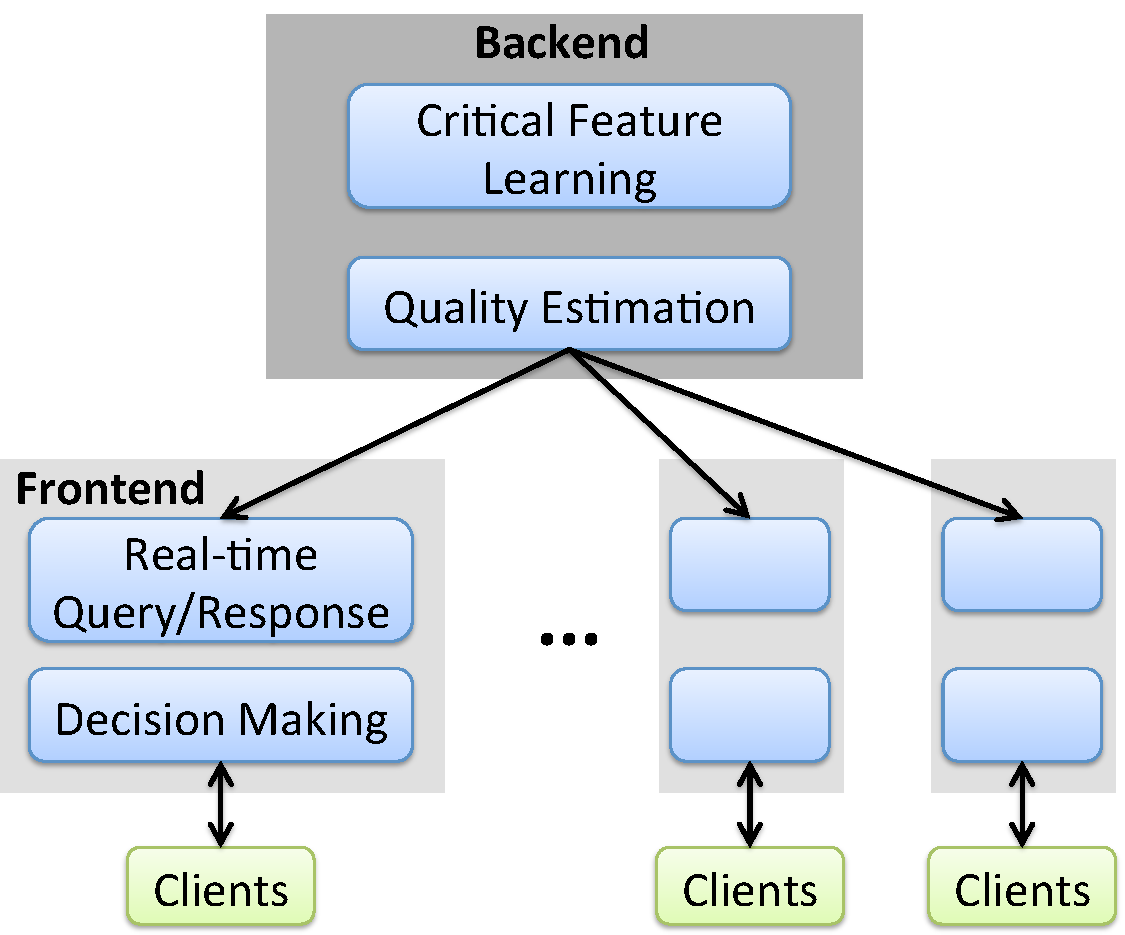
\includegraphics[width=.55\textwidth]{figures/cfa-impl-overview.pdf}
\vspace{-0.1cm}
\caption{Implementation overview of \dda. The three stages of 
\dda workflow are implemented in a backend cluster and distribute
frontend clusters.}
%\vspace{-0.2cm}
\label{fig:impl}
\end{figure}

\mypara{Centralized backend} 
The critical feature learning and quality 
estimation stages are implemented in a backend 
cluster as periodic jobs. 
By default, critical feature learning runs every 30 
minutes, and quality estimation runs every minute. 
A centralized backend is a natural choice because 
we need  a global view of all quality measurements.
The quality function, once updated by the estimation 
step, is disseminated to distributed 
frontend clusters using Kafka~\cite{kreps2011kafka}.

%backend cluster is two-fold.
%First, the backend has the access to the database of 
%all quality measurements, which is needed by critical 
%feature learning and quality estimation.
%Second, they are not required to be as much responsive to client 
%requests as real-time query/response. 

%For real-time query/response to use the up-to-date 
%quality function (i.e., a map between a \leaf and 
%quality estimation), 

Note that we can further reduce learning time
 using simple parallelization strategies. 
%(As discussed in \Section\ref{subsec:scalability}, parallelization alone does not provide a scalable workflow).  
Specifically, the critical features of different \leafs 
can be learned independently.
Similarly in Algorithm~\ref{alg:learning}, the 
similarity  of quality distributions can be 
computed in parallel. 
To exploit this data-level parallelism, 
we implement them as Spark jobs~\cite{spark}. 



\mypara{Distributed frontend} 
%Real-time query/response to prediction queries 
%is implemented in distributed frontend clusters, 
%where decision makers  (which selects CDN, 
%bitrate for clients) are located~\cite{c3}.
Real-time query/response and 
decision makers of CDN/bitrate are co-located in 
distributed frontend clusters that are closer to 
clients than the backend.
%Pushing real-time query/response and 
%decision maker to distributed frontend 
Each frontend cluster receives the quality function 
from the backend and caches it locally for fast
prediction.
This reduces the latency of making decisions 
for clients.
 




%The learning of critical feature function and quality 
%functions on different ``\leafs'' is independent. 
%Critical feature learning can simultaneously 
%evaluate the distribution similarity in 
%Algorithm~\ref{alg:learning} of multiple feature 
%combinations in one ``Map'' operation and find the 
%critical feature in one ``Reduce'' operation. 
%To exploit such parallelism, these two stages are 
%implemented as Spark MapReduce jobs~\cite{spark}. 



\subsection{Challenges in an Operational Setting}
\label{subsec:cfa:impl:challenge}

%Next, we highlight some operational experience from the 
%deployment of \dda in a production system.

\mypara{Mitigating impact of bulk data loading} 
%Resources, such as bandwidth and cluster nodes 
%(sender/receivers) between the quality measurement 
%database and 
The backend cluster is shared 
and runs other delay-sensitive 
jobs; e.g.,  analytics queries from production teams. 
 Since the critical feature learning runs periodically 
and loads a large amount of data ($\approx$30 
GB), it creates spikes in the delays of other jobs 
(Figure~\ref{fig:completion-delay}).  
To address this concern, we engineered a simple 
heuristic to evenly spread the data retrieval where  
we load a small piece of data every few minutes. 
As Figure~\ref{fig:completion-delay} shows, this 
reduces the spikes caused by bulk data loading in 
batch mode.
Note that this does not affect critical feature learning.


\begin{figure}[t!]
\centering
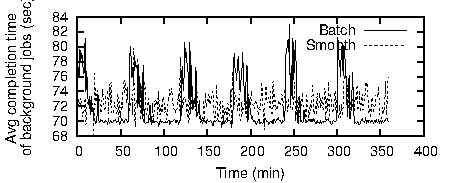
\includegraphics[width=.8\textwidth]{figures/cfa-smooth-batch-timeseries.pdf}
%\vspace{-0.3cm}
\caption{Streaming data loading has smoother 
impact on completion delay than batch data loading.}
%\vspace{-0.4cm}
\label{fig:completion-delay}
\end{figure}

\mypara{Iterative algorithm refinement}
Some parameters (e.g., learning window size 
\HTimeWindowLearn) of \dda require iterative tuning in a 
production environment.
%However, one practical challenge arises  due to code release cycles.
However, one practical challenge is that the 
frontend-facing part of the backend can 
only  be updated once every couple of weeks 
due to code release cycles. 
Thus,  rolling out new prediction algorithms may 
take several days and is a practical concern.
Fortunately, the decoupling between critical feature 
learning and quality estimation 
(Section~\ref{subsec:scalability})
means that changes to critical feature learning
are confined to the backend cluster. 
This enables us to rapidly refine 
and customize the \dda algorithm. 
% (Without this decoupling, any changes to \dda 
%would also need to update quality estimation in the front-end facing part of
%the backend, and would be have slow refresh cycles.)



\section{Evaluation}
\label{sec:cfa:eval}


In this section, we show that:
\begin{packeditemize}
\item \dda  predicts video quality with 30\% less error than 
competing machine learning algorithms 
(Section~\ref{subsec:eval-accuracy}).
\item Using \dda-based prediction, we can improve  
video quality significantly; e.g., 32\% less BufRatio, 
12\% higher AvgBitrate in a pilot deployment 
(Section~\ref{subsec:eval-improvement}).
% than those selected by a baseline players. 
%More extensive trace-driven simulation shows that across different quality metrics, \dda leads to 5-17\% improvement over decisions made by the more accurate prediction algorithms other than \dda.
\item \dda is responsive to client  queries and  makes 
predictions based on the most recent critical features 
and quality measurements 
(Section~\ref{subsec:eval-scalability}).
\end{packeditemize}


%\begin{figure*}[t!]
%\centering
%\hspace{-0.5cm}
%\subfigure[Distribution of per-session prediction error]
%{
%        \includegraphics[width=0.5\textwidth]{eval-figs/batch-3/barchart-distribution.pdf}
%        \label{subfig:per-session-error}
%}
%\hspace{-0.3cm}
%\subfigure[Kendall rank correlation coefficient]
%{
%         \includegraphics[width=0.5\textwidth]{eval-figs/batch-3/barchart-correlation.pdf}
%        \label{subfig:kendall}
%}
%\hspace{-0.5cm}
%\vspace{-0.3cm}
%\tightcaption{Compared with conventional machine learning techniques (green) and naive prediction algorithms (blue), \dda can accurately predict each session's quality and the rank between different quality values (Kendall coefficient).}
%\vspace{-0.3cm}
%\label{fig:accuracy}
%\end{figure*}


\begin{figure}[t!]
\centering
%\hspace{-0.6cm}
\subfloat[AvgBitrate]
{
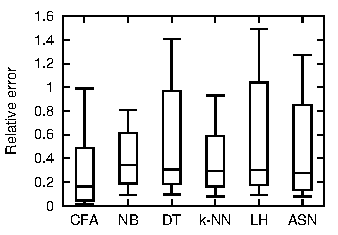
\includegraphics[width=.4\textwidth]{figures/cfa-barchart-distribution-AvgBitrate.pdf}
        \label{subfig:accuracy-avgbitrate}
}
%\hspace{-0.4cm}
\subfloat[JoinTime]
{
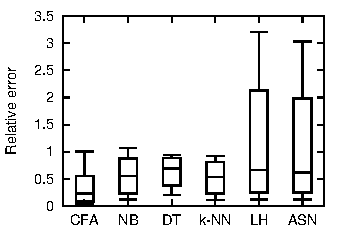
\includegraphics[width=.4\textwidth]{figures/cfa-barchart-distribution-JoinTime.pdf}
        \label{subfig:accuracy-avgbitrate}
}
%\hspace{-0.6cm}
\\
%\vspace{-0.25cm}
%\hspace{-1cm}
\subfloat[BufRatio]
{
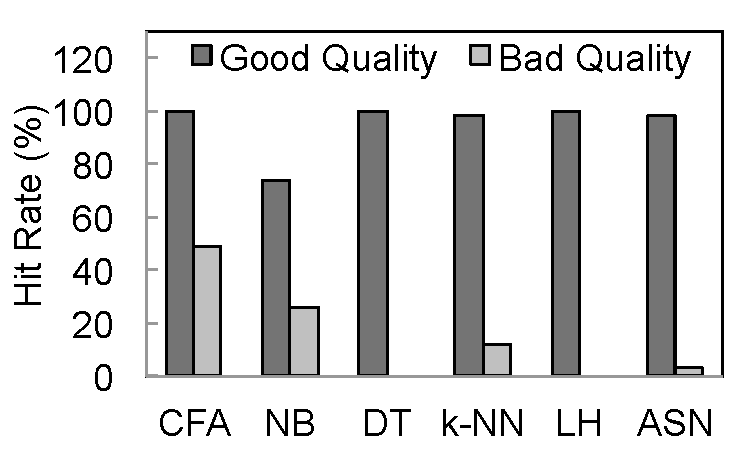
\includegraphics[width=.4\textwidth]{figures/cfa-HitRate-BufRatio.pdf}
        \label{subfig:accuracy-bufratio}
}
%\hspace{-0.4cm}
\subfloat[VSF]
{
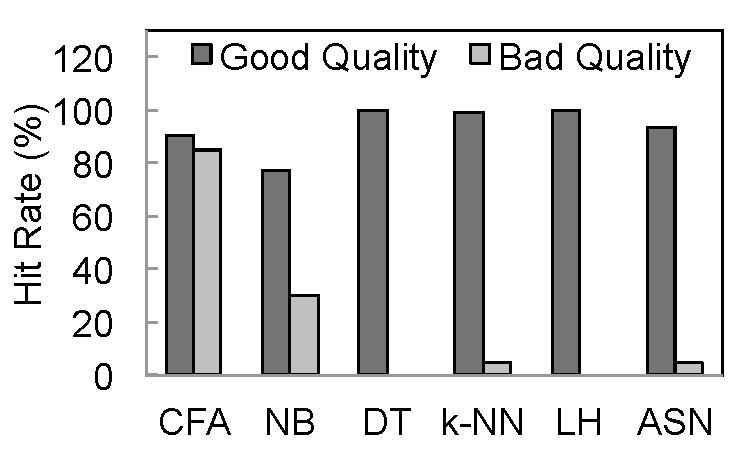
\includegraphics[width=.4\textwidth]{figures/cfa-HitRate-VSF.pdf}
        \label{subfig:accuracy-vsf}
}
\caption{Distributions of relative prediction error ($\{5,10,50,90,95\}\%$iles) on AvgBitrate and JoinTime and hit rates on BufRatio and VSF. They show that \dda outperforms other algorithms.}
%\vspace{-0.3cm}
\label{fig:accuracy}
\end{figure}

\subsection{Prediction Accuracy}
\label{subsec:eval-accuracy}
We compare \dda with five alternative algorithms: three
simple ML algorithms, Naive Bayes (NB), Decision Tree (DT),
$k$-Nearest Neighbor ($k$-NN)\footnote{NB, DT, and 
$k$-NN are mplemented using a popular ML
library \texttt{weka}\cite{weka}.}, and two heuristics 
 which predict a session's quality by the average quality 
of other sessions from the same ASN (ASN) or matching 
the last-mile connection type (LH). 
All algorithms use the same set of features listed in 
Table~\ref{tab:features}.


%First, we show that \dda yields high prediction accuracy. 

Ideally, we want to evaluate how accurately an algorithm 
can predict the quality of a given client on every choice 
of CDN and bitrate. 
However,  this is infeasible since each video client is 
assigned to only one CDN and bitrate at any time.
Thus,  we  can only evaluate the prediction accuracy 
over the observed CDN-bitrate choices, and we use the 
quality measured on these choices as the ground truth.
%A caveat of this methodology is that it evaluates the accuracy only over decisions of bitrate and CDN that were actually made.%; i.e., the error is not over the entire space of decisions. 
That said, this approach is still useful for doing a relative 
comparison across different algorithms.  

%\myparatight{Per-session prediction error} 
For AvgBitrate and JoinTime, we report {\em relative error}:
$\frac{|p-q|}{q}$, where the $q$ is the ground truth and 
$p$ is the prediction.
For  BufRatio and JoinTime, which have more ``step 
function'' like effects~\cite{sigcomm11}, we report a 
slightly different measure called {\em hit rate}:
how likely a session with good quality (i.e., 
BufRatio~$<5\%$, VSF=0) or bad quality is correctly 
identified. 
%We compare the prediction accuracy over 20 millions sessions from a real dataset of a week.
Figure~\ref{fig:accuracy} shows that for AvgBitrate and
JoinTime, \dda has the lowest $\{5,10,50,90\}\%$th 
percentiles of prediction error and lower $95\%$th 
percentiles than most algorithms.  
In particular, median error of \dda is about 30\% lower 
than the best competing  algorithm.  
In terms of BufRatio and VSF, \dda significantly 
outperforms other algorithms in the hit rate of bad 
quality sessions. 
The reason  for hit rate of bad quality to be lower than 
that of good quality is that bad quality sessions are 
almost always less than good quality, which makes 
them hard to predict.
Note that accurately identifying sessions that have bad 
quality is crucial as they have the most room for 
improvement.


%\myparatight{Rank correlation} In addition to prediction error, it is also useful to quantify whether the prediction algorithm can accurately identify the {\em rank} of two quality values. To this end, we calculate the Kendall rank correlation coefficient between actual and predicted quality of different algorithms. 
%%To ensure the rank is meaningful, we exclude duplicated actual quality. 
%Figure~\ref{subfig:kendall} shows that \dda has much higher Kendall rank correlation coefficient than the five strawman algorithms, which means \dda can better differentiate different quality values.
%An interesting observation is that \dda has more advantages on BufRatio and VSF, where \dda does not have much better prediction error in Figure~\ref{subfig:per-session-error}. This is because most values of BufRatio and VSF are zero (i.e., no extra buffering or no start failure). While most algorithms can easily achieve low error on these zero values, it is hard for them to predict other values accurately.



\subsection{Quality Improvement}
\label{subsec:eval-improvement}

%Next, we show that CDN and bitrate selected based on quality prediction of \dda leads to better quality than baseline approaches. We show it by a real-world pilot deployment as well as real-world trace-driven simulation.


\mypara{Pilot deployment}
As a pilot deployment, we integrated \dda in a production 
system that provides a global video optimization 
service~\cite{c3}.
% that manages delivery for several premium band content providers.  
We deployed \dda on one major content provider and used it 
 to optimize 150,000 sessions each day.
% by selecting among 3 CDNs and 6 bitrates.
%To demonstrate the improvement using \dda, 
We ran an A/B test (where each algorithm was used on 
a random subset of clients) to  evaluate the improvement 
of \dda over a baseline random decision maker, which 
many video optimization services  use by default (modulo 
business arrangement like price)~\cite{hulu}.
%\footnote{\dda is also better than the custom  algorithm 
% used in production. Due to proprietary concerns, we do not show quantitative results vs.\  production strategies.
%\camera{Qualitatively, \dda is automated while the custom algorithm has had several rounds of manual tweaking, so the fact that \dda is better is already promising. Furthermore, conversations with engineers were positive, and they were willing to invest time in implementing \dda and running longer pilots.}  }



\begin{table}[t!]
\begin{center}
%\begin{small}
\begin{tabular}{l|c|c|c}
 & \dda & Baseline & Improvement \\ \hline \hline
QoE & 155.43 & 138.27 & 12.4\% \\
BufRatio & 0.0123 & 0.0182 & 32\% \\ 
AvgBitrate & 3200 & 2849 & 12.31\% \\
\end{tabular}
%\end{small}
%\vspace{-0.2cm}
\caption{Random A/B testing results of \dda vs. baseline in 
real-world deployment.}
%\vspace{-0.2cm}
%\vspace{-0.4cm}
\label{tab:pilot-statistics}
\end{center}
\end{table}


\begin{figure*}[t!]
\centering
\subfloat[\dda vs.\ baseline by time]
{
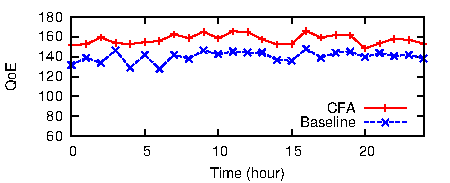
\includegraphics[width=.7\textwidth]{figures/cfa-realimp-timeseries--1.pdf}
        \label{subfig:per-session-error}
}\\
%\hspace{-0.8cm}
\subfloat[\dda vs.\ baseline by spatial partitions]
{
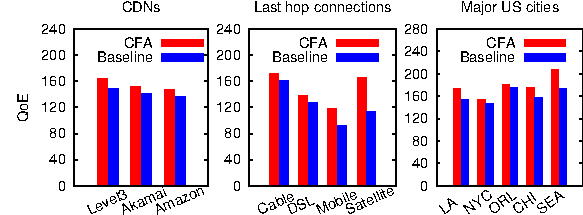
\includegraphics[width=.8\textwidth]{figures/cfa-realimp-bar-partitions--1.pdf}
        \label{subfig:real-world-spatial}
}
%\vspace{-0.3cm}
\caption{Results of real-world deployment. 
\dda outperforms the baseline random decision maker 
(over time and across different large cities, connection t
ypes and CDNs).}
%\vspace{-0.4cm}
\label{fig:real-world-improvement}
\end{figure*}


Table~\ref{tab:pilot-statistics} compares \dda with the 
baseline random decision maker in terms of the mean 
BufRatio, AvgBitrate
%\footnote{JoinTime and VSF are not shown as they are not explicitly optimized} 
and a simple QoE model 
($QoE=-370*BufRatio+AvgBitrate/20$), which was 
suggested by~\cite{sigcomm12conviva,sigcomm11}. 
Over all sessions in the A/B testing, \dda shows an 
improvement in both BufRatio (32\% reduction) and 
AvgBitrate (12.3\% increase) compared to the baseline.
This shows that \dda is able to simultaneously optimize
multiple (possibly conflicting) metrics. 
To put these numbers in context, our conversation 
with domain experts  confirmed that these 
improvements are significant for content providers and 
 can potentially translate into  substantial benefits in 
 engagement and revenues~\cite{convivapersonal}.
% \dda's superior performance and our conversations with domain experts indicate that they were willing to invest time running longer pilot.
\dda's superior performance and that  \dda is more 
automated than the custom algorithm indicate that 
domain experts were willing to invest time running 
longer pilot.
Figure~\ref{fig:real-world-improvement} provides 
more comparison and shows that \dda consistently 
outperforms the baseline over time and across different 
major cities in the US, connection types and CDNs. 
%Especially, quality of each CDN is improved, which means quality can be 
%improved by only selecting bitrate based on \dda prediction.


%\vyas{where are the numbers in 6.0 coming from??}


\mypara{Trace-driven simulation}
%While real-world deployment is realistic, it has inherent constraints such as load of CDNs (e.g., in the pilot deployment, the traffic assigned to each CDN needs to be within a lower and upper bound due to business contract), and limited scalability to simultaneously evaluate many instantiations of prediction systems. 
%Trace-driven evaluation may address these constraints, but it needs to estimate the quality of decisions that had not been used. 
We complement this real-world deployment with a 
trace-driven simulation to simultaneously compare 
more algorithms over more quality metrics. 
However, one key challenge is that it is hard to 
estimate the quality of a decision that was not used 
by a specific client in the trace.

To address this problem, we use the 
{\em counterfactual methodology} from prior work in 
online recommendation 
systems~\cite{li2010contextual,li2011unbiased}.
Suppose we have quality measurements from a 
set of clients,
where client $c$ is assigned to a decision $d_{rand}(c)$ 
of CDN and bitrate at random.
Now, we have a new hypothetical algorithm that maps 
client $c$ to $d_{alg}(c)$. 
Then, we can evaluate the average quality of clients 
assigned to each decision $d$,  $\{c|d_{alg}(c)=d\}$, 
by the average quality of $\{c|d_{alg}(c)=d,d_{rand}(c)=d\}$.
Finally, the average quality of the new algorithm is 
the weighted sum of average quality of all decisions, 
where the weight of each decision is the fraction of 
sessions assigned to it.
% being randomly assigned to a decision (CDN and bitrate).
%Then, to evaluate a different assignment between the same clients and decisions, 
%we can estimate the average quality of each decision in the 
%new assignment by the average quality of the clients that are assigned 
%to this decision in both new assignment and the previous random assignment.
This can be proved to be an unbiased (offline) 
estimate of $d_{alg}$'s (online) 
performance~\cite{cfe-report}.\footnote{One known 
limitation of this analysis is that it assumes the new 
assignments do not affect each decision's overall 
performance. 
For instance, if we assign all sessions to one CDN, 
they may overload the CDN and so this CDN's quality 
in the random assignments is no longer useful. 
Since this work only focuses on controlling traffic at a 
small scale relative to the total load on the CDN (and 
our experiments are in fact performed at such a scale), 
this methodology is still unbiased.}
For instance, if out of 1000 clients assigned to use 
Akamai and 500Kbps, 200 clients are assigned to this 
decision in the random assignment, then we can use 
the average quality of these 200 sessions as an unbiased
estimate of the average quality of these 1000 sessions.
%for each decision (i.e., a specific CDN and bitrate), we first randomly select a subset of client to use the decision (i.e., the selection is independent to any aspect of a client). Then, given a new assignment of the same clients, for each decision, the subset of client that are assigned to this decision in both random assignment and new assignment represents an unbiased estimation of average quality of this decision in the new assignment. 
%It can be proved to be an {\em unbiased} estimate of average quality of 
%any new decision assignment\footnote{}.
%For a proof, please refer~\cite{cfe-report}.
Fortunately, our dataset includes a (randomly chosen) 
portion of clients with randomized decision assignments 
(i.e., CDN and bitrate). 
Thus, we  only report improvements  for these clients. 
 %such content providers and restrict the evaluation  to these clients.



\begin{figure}[t!]
\centering
%\hspace{-0.4cm}
%\subfigure[QoE]
%{
%\includegraphics[width=.2\textwidth]{eval-figs/batch-3/cfImp--1.pdf}
%        \label{subfig:Imp-cfImp--1}
%}
%\hspace{-0.4cm}
%\subfigure[BufRatio]
%{
%\includegraphics[width=.2\textwidth]{eval-figs/batch-3/cfImp-0.pdf}
%        \label{subfig:Imp-cfImp-0}
%}
%\hspace{-0.4cm}
%\subfigure[AvgBitrate]
%{
%\includegraphics[width=.2\textwidth]{eval-figs/batch-3/cfImp-1.pdf}
%        \label{subfig:Imp-cfImp-1}
%}
%\hspace{-0.4cm}
%\subfigure[JoinTime]
%{
%\includegraphics[width=.2\textwidth]{eval-figs/batch-3/cfImp-2.pdf}
%        \label{subfig:Imp-cfImp-2}
%}
%\hspace{-0.4cm}
%\subfigure[VSF]
%{
%\includegraphics[width=.2\textwidth]{eval-figs/batch-3/cfImp-3.pdf}
%        \label{subfig:Imp-cfImp-3}
%}
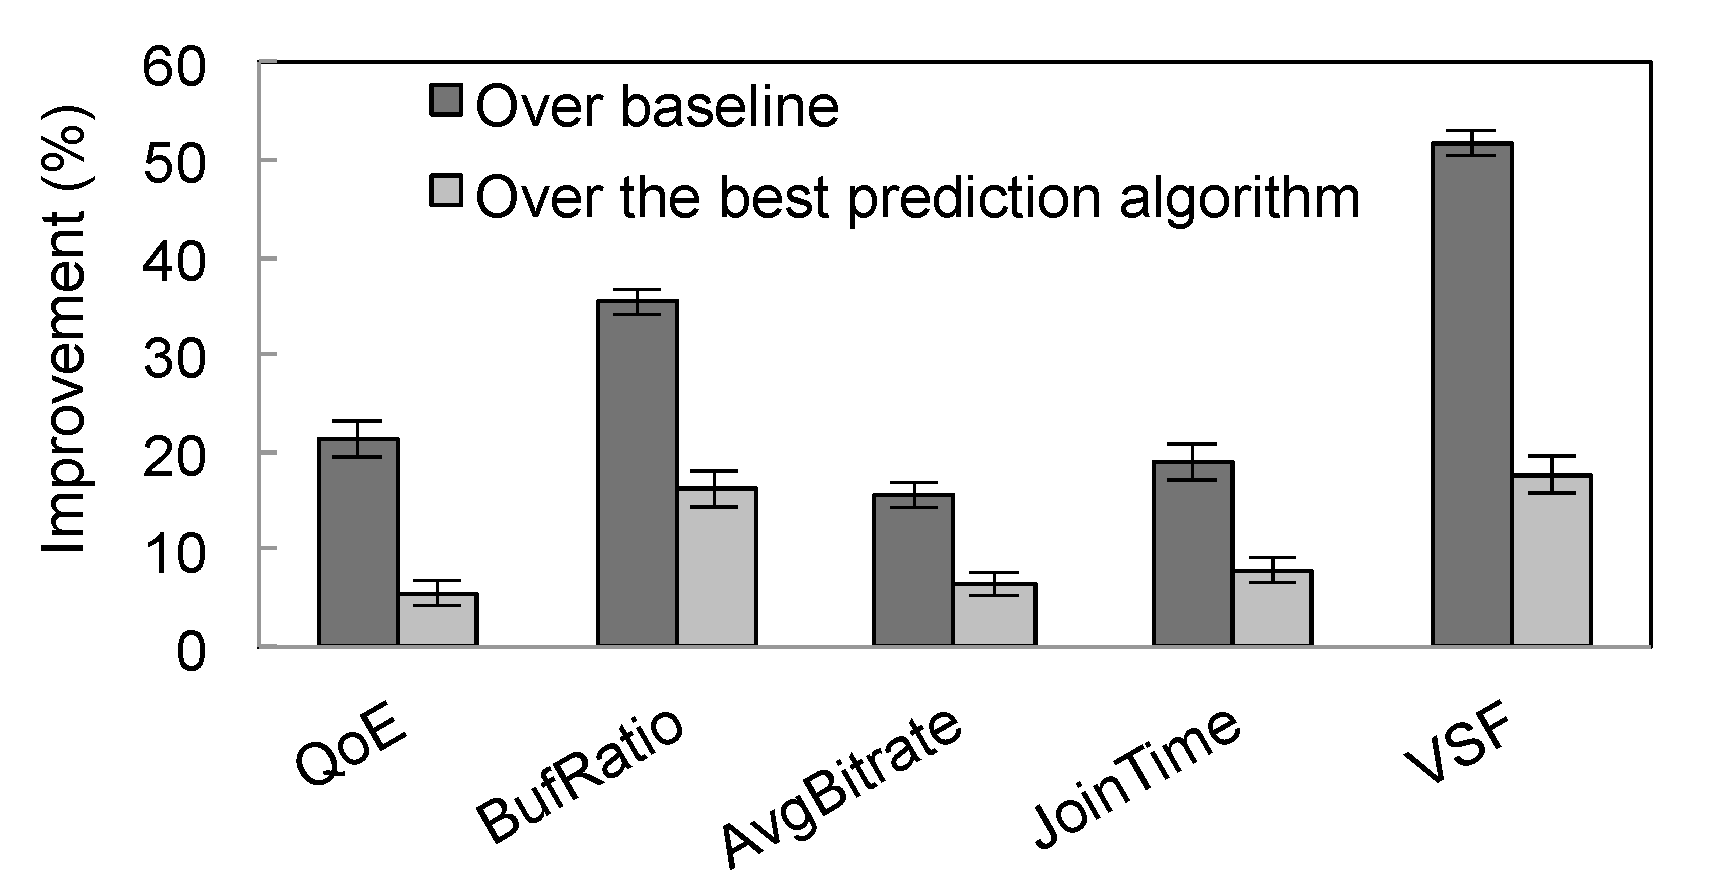
\includegraphics[width=0.65\textwidth]{figures/cfa-CF-IMPROVEMENT-Perc-Grouped.pdf}
%\vspace{-0.3cm}
\caption{Comparison of quality improvement 
between \dda and strawmen.}
%\vspace{-0.3cm}
\label{fig:trace-driven-improvement}
\end{figure}


Figure~\ref{fig:trace-driven-improvement} uses this 
counterfactual methodology and compares \dda with the 
best alternative from Section~\ref{subsec:eval-accuracy} for 
each quality metric and the baseline random decision 
maker (e.g., the best alternative of AvgBitrate is k-NN). 
For each quality metric and prediction algorithm, the 
decision maker selects the CDN and bitrate that has 
the  best predicted quality for each client. 
For instance, the improvement of \dda over the baseline 
on VSF is 52\% -- this means the number of sessions 
with start failures is 52\% less than when the baseline 
algorithm is used.
The figures show that \dda outperforms the baseline 
algorithm by 15\%-52\%. 
They also show that \dda outperforms the best prediction 
algorithms by 5\%-17\%. %\vyas{make numbers consistent with 6.0 and intro}



\subsection{Timeliness of Prediction}
\label{subsec:eval-scalability}

Our implementation of \dda should
(1) retain freshness to minimize the impact of staleness on prediction accuracy, and 
(2) be responsive to each prediction query. 




\begin{figure}[t!]
\centering
%\hspace{-0.6cm}
\subfloat[BufRatio]
{
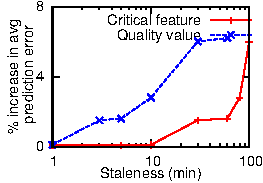
\includegraphics[width=.4\textwidth]{figures/cfa-insight-staleness-impact-0.pdf}
        \label{subfig:Imp-cfImp--1}
}
%\hspace{-0.4cm}
\subfloat[AvgBitrate]
{
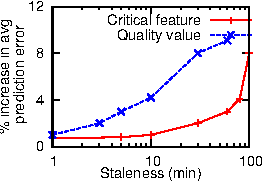
\includegraphics[width=.4\textwidth]{figures/cfa-insight-staleness-impact-1.pdf}
        \label{subfig:Imp-cfImp-0}
}
%\hspace{-0.6cm}
\\
%\vspace{-0.2cm}
%\hspace{-1cm}
\subfloat[JoinTime]
{
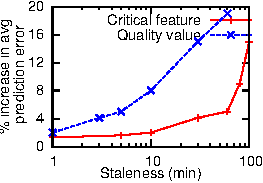
\includegraphics[width=.4\textwidth]{figures/cfa-insight-staleness-impact-2.pdf}
        \label{subfig:Imp-cfImp-1}
}
%\hspace{-0.4cm}
\subfloat[VSF]
{
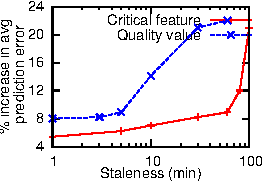
\includegraphics[width=.4\textwidth]{figures/cfa-insight-staleness-impact-3.pdf}
        \label{subfig:Imp-cfImp-2}
}
%\hspace{-0.6cm}
%\vspace{-0.3cm}
\caption{Latency of critical features and quality values 
(x-axis) on increase in accuracy (y-axis).}
%\vspace{-0.2cm}
\label{fig:insight-staleness}
\end{figure}


\begin{table}[t!]
\begin{center}
%\begin{small}
\begin{tabular}{p{2in}|p{2in}|p{2in}}
{\bf Stage} & {\bf Run time (mean / median)} & {\bf Required freshness} \\ \hline \hline
Critical feature learning & 30.1/29.5 min & 30-60 min \\
Quality estimation  &  30.7/28.5 sec & 1-5 min \\
Query response	 &  0.66/0.62 ms & 1 ms
\end{tabular}
%\end{small}
\caption{Each stage of \dda is refreshed to meet the 
required freshness of its results.}
\label{tab:response-all}
\end{center}
%\vspace{-0.7cm}
\end{table}


We begin by showing how fast each stage described 
in Section~\ref{subsec:scalability} needs to be refreshed. 
Figure~\ref{fig:insight-staleness} shows the impact of 
staleness of critical features and quality values on the 
prediction accuracy of \dda. 
First, critical features learned 30-60 minutes before 
prediction can still achieve similar accuracy as those 
learned 1 minute before prediction. 
In contrast, quality estimation cannot be more than 
10 minutes prior to when prediction is made (which 
corroborates the results of 
Figure~\ref{fig:strawman-staleness-all-metrics}). 
Thus, critical feature learning needs to be refreshed 
every 30-60 minutes and quality estimation should be 
refreshed at least every several minutes. 
Finally, prediction queries need to be responded to within 
several milliseconds~\cite{c3} (ignoring network delay 
between clients and servers).




Next, we benchmark the time to run each logical stage 
described in Section~\ref{subsec:scalability}.
Real-time query/response runs in 4 geographically 
distributed data centers.
Critical feature learning and quality estimation run 
on two clusters of 32 cores. 
Table~\ref{tab:response-all} shows the time for 
running each stage and the timescale required to 
ensure freshness. 
It confirms that the implementation of \dda is sufficient 
to ensure the freshness of results in each stage.



\section{Insights from Critical Features}
\label{sec:cfa:insight}

%In this section, we use the set of critical features learned by \dda from real data 
% to shed 
% light on interesting observations on video quality.  This analysis suggests that, 
In addition to the predictive power, \dda also offers 
 insights into the ``structure'' of video quality in the wild. 
%(unlike, say, complex projections 
% like PCA or SVM). 
In this section, we  focus on two questions:
(1) What types of critical features are most common?
(2) What factors have significant impact on video quality?

\subsection{Types of Critical Features} 
\label{subsec:insight-type}


\mypara{Popular types of critical features} 
Figure~\ref{fig:insight-type} shows a breakdown of the 
fraction of sessions that are assigned to a specific 
type of critical feature set. We show this for  different 
quality metrics. 
(Since we focus on a specific VoD provider, we do 
not consider the \fSite or \fLiveOrVoD for this analysis.)
Across all quality metrics, the most popular critical 
features are \fCDN, \fASN and \fConnectionType, which 
means video quality is greatly impacted by network 
conditions at the server (\fCDN), transit network (\fASN),
and last-mile connection (\fConnectionType).  

\begin{figure}[t!]
\centering
%\hspace{-0.6cm}
\subfloat[BufRatio]
{
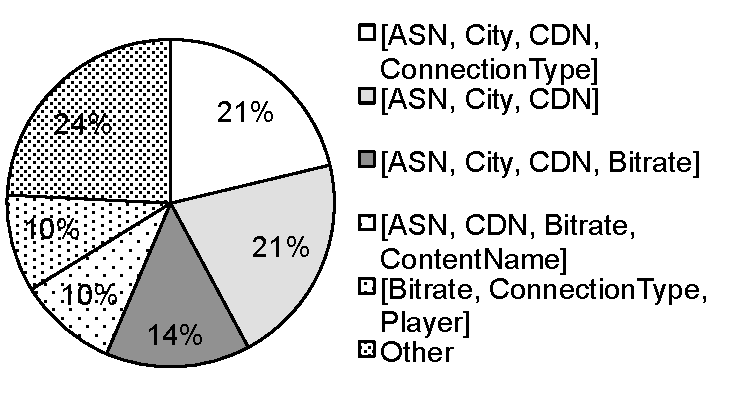
\includegraphics[width=.47\textwidth]{figures/cfa-insight-type-0.pdf}
        \label{subfig:insight-type-0}
}
%\hspace{-0.4cm}
\subfloat[AvgBitrate]
{
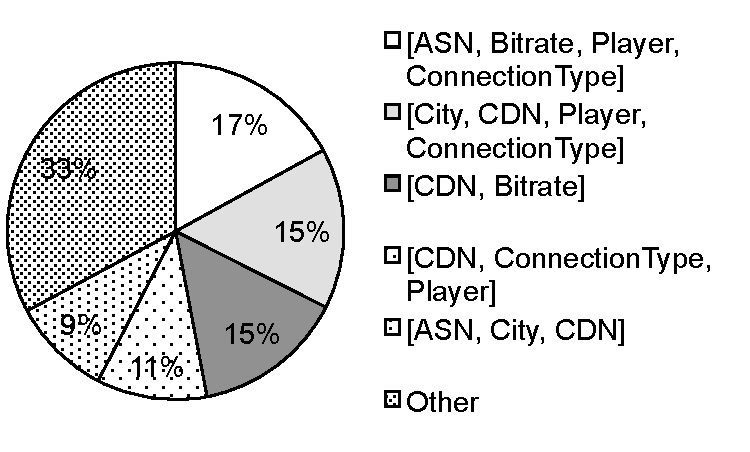
\includegraphics[width=.47\textwidth]{figures/cfa-insight-type-1.pdf}
        \label{subfig:insight-type-1}
}
%\hspace{-0.6cm}
\\
%\hspace{-1cm}
\subfloat[JoinTime]
{
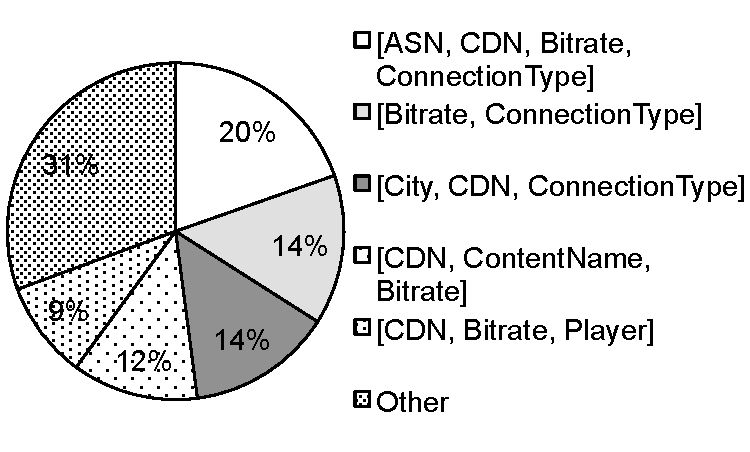
\includegraphics[width=.47\textwidth]{figures/cfa-insight-type-2.pdf}
        \label{subfig:insight-type-2}
}
%\hspace{-0.4cm}
\subfloat[VSF]
{
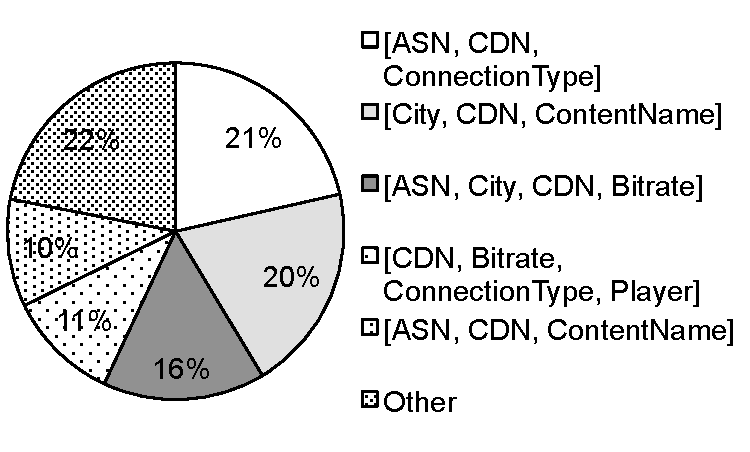
\includegraphics[width=.47\textwidth]{figures/cfa-insight-type-3.pdf}
        \label{subfig:insight-type-3}
}
%\hspace{-0.6cm}
%\vspace{-0.3cm}
\caption{Analyzing the types of critical features: This shows a 
breakdown of the total number of sessions assigned to a 
specific type of critical features.}
%\vspace{-0.3cm}
\label{fig:insight-type}
\end{figure}

We also see  interesting patterns unique to individual metrics.
\fCity is among the top critical features of BufRatio. This is perhaps because network
congestion usually depends on the volume of concurrent viewers in a specific
region.  \fBitrate (initial bitrate) has a larger impact on AvgBitrate than
on other metrics, since the videos in the dataset are mostly short content
(2-5 minutes) and AvgBitrate is correlated with initial bitrate. 
 Finally, \fContentName has a relatively large impact on failures (VSF) but not 
 other metrics, because VSF is sometimes due to the requested content not being ready. 

%Remember in \Section\ref{sec:insights} that there could be more critical

\myparatight{Distribution of types of critical features} 
%From the critical features that we learned, 
While the quality of about 50\% of sessions is impacted by
3-4 popular types of critical features, 15\% of sessions are
 impacted by a diverse set of more than 30 types of critical feature (not shown).  
This corroborates the need for expressive prediction models that handle the diverse
factors affecting quality (Section~\ref{subsec:expressive}). %\vyas{i cant parse this sentence}


\subsection{Values of Critical Features}
\label{subsec:insight-value}

%\comment
%{
%\myparatight{Real-world events revealed by critical feature values}
%We show that the real example of high dimensionality (\Section\ref{subsec:expressive}) can be revealed by values of critical features.
%%a confirmed one-day event when many Maryland Comcast users suffered from high VSF when accessing Level3.
%We find that 81\% of sessions using Comcast in Baltimore have $\fCDN=Level3$, $\fASN=7922$ (i.e., ``Comcast'') and $\fCity=Baltimore$ as values of critical features. 
%In contrast, only 17\% of other sessions (e.g., Verizon users in Maryland or Comcast users in California) have $CDN$, $ASN$ and $City$ as (part of) critical features. 
%%This shows that factors affecting video quality can be really reflected by the values of critical features.
%}

Next, we focus on the most prevalent {\em feature values} 
(e.g., a specific ASN or player).  
To this end, we define {\em prevalence} of a feature value  
by the fraction of video sessions matching this feature value 
that have this feature as one of their critical features; e.g., 
the fraction of video sessions from Boston that have \fCity
as one of their critical features.
If a feature value has a large prevalence, then the  quality 
of many  sessions that have this feature value can be 
explained by this feature.


%\myparatight{Most prevalent values of critical features}


%Note that the definition of prevalence is independent to the total population of sessions with a specific feature value (i.e., a small ISP can have a large prevalence if most of its sessions have its ASN as critical feature).
%In other words, what feature values have the highest impact on video quality if a session has it.

We present the values of critical features with a prevalence 
higher than 50\% for each quality metric and 
only consider a subset of the features ($ASN$, $City$, 
$ContentName$, $ConnectionType$) that appear 
prominently in  Figure~\ref{fig:insight-type}.  
We present this analysis with two caveats.  
First, due to proprietary concerns, we do not present 
the names of the entities, but focus on their characteristics.  
Second, we cannot confirm some of our hypothesis as it 
involves other  providers;  as such, we intend this result 
to be illustrative rather than conclusive. 

\begin{table}[t!]
%\begin{footnotesize}
\begin{tabular}{p{2.0cm}|p{3cm}|p{3cm}|p{3cm}|p{3cm}}
   &\textbf{$City$} & \textbf{$ASN$} & \textbf{$Player$} & \textbf{$ConnectionType$}\\ \hline \hline
BufRatio & Some major east-coast cities & & & Satellite, Mobile, Cable \\ \hline
AvgBitrate & & Cellular carriers & Players with different encodings & \\ \hline
JoinTime &  & Cellular carrier & & Satellite, DSL \\ \hline
VSF & & Small ISPs & & Satellite, Mobile \\
\end{tabular}
%\end{footnotesize}
%\vspace{-0.1cm}
\caption{Analysis of the most prevalent values of critical features. 
A empty cell implies that we found no interesting values in this combination.}
%\vspace{-0.2cm}
\label{tab:insight-popular-values}
\end{table}

Table~\ref{tab:insight-popular-values} presents some
anecdotal examples we observed.  
In terms of BufRatio, we see some of the major east 
coast cities (e.g., Boston, Baltimore) are more likely to be 
critical feature values than other smaller cities.  
We also see both poor (Satellite, Mobile) and broadband 
(Cable) connection types have high prevalence on 
BufRatio and JoinTime.  
This is because poor quality sessions are bottlenecked 
by poor connections, while some good quality sessions 
are explained by their broadband connections.  
``Player'' has a relatively large prevalence on AvgBitrate, 
because the content provider uses different  bitrate levels 
for different players (Flash or iOS).  
Finally, in terms of VSF, some small ISPs have large 
prevalence.  We speculate that this is because
their peering relationships with major CDNs are not 
provisioned, so their video sessions have relatively 
high failure rates.
%Cellular carriers have large impact on AvgBitrate and JoinTime, which are
%directly bottlenecked by available bandwidth.

%It is a bit surprising that there are also a few German cities (e.g., Berlin) and ISPs



\section{Discussion}
\label{sec:cfa:discuss}

\mypara{Relationship to existing ML techniques}
\dda is a domain-specific prediction system that 
outperforms some canonical ML algorithms 
(Section~\ref{subsec:eval-accuracy}). 
We put \dda in the context of three types of 
ML algorithms.
\begin{packeditemize}
%\item Multi-armed bandit techniques attempt to identify the decision with the highest reward among multiple choices, and we believe they are complementary to \dda. The multi-armed bandit problem assumes that each decision has a fixed distribution of rewards, which is not true since video quality also depends on client-side features. In the meantime, one concern of \dda is that predictions based on quality measurements from clients may be biased by previous decisions. An interesting future work is to use multi-armed bandit techniques over the video client that share the same critical features.
\item {\em Multi-armed bandit} algorithms~\cite{mab} 
find the decision with the highest reward (i.e., best 
CDN and bitrate) from multiple choices. 
They assume each decision has a fixed distribution 
of rewards, but the video quality of a CDN also 
depends on client-side features.
In contrast, contextual multi-armed bandit 
algorithms~\cite{cmab} assume the best decision 
depends on contextual information, but they require 
appropriate modeling between the context and 
decision space, to which critical features provide 
one viable approach.
\item {\em The feature selection} 
problem~\cite{feature-selection} seems similar to 
critical feature learning, but with a key difference: 
critical features vary across video sessions. 
Thus, techniques looking for features that are most 
important for all sessions are not directly applicable.
\item {\em Advanced ML} algorithms today can 
handle highly complex models~\cite{deeplearning, svm} 
efficiently, so in theory the critical features could be 
automatically identified, albeit in an implicit manner. 
\dda uses existing ML models (specifically, the ``variable 
kernel conditional density estimation'' 
method~\cite{terrell1992variable}) and may be less 
accurate than advanced ML techniques, but \dda can 
predict with more recent data since it tolerates stale 
update on the critical features. Furthermore, \dda is 
less opaque since it is based on domain-specific 
insights about critical features (Section~\ref{sec:cfa:outline}). 
%Though advanced ML techniques might be more accurate, we believe \dda is more scalable since it tolerates staled update on the critical features. 
\end{packeditemize}

\mypara{Prediction and selection bias}
One concern of making predictions and decisions 
based on quality measurements from clients is that 
they may be biased by previous decisions. 
For instance, if we move all video clients to the 
current optimal decision, we would not be able to 
predict quality on other decisions (i.e., a classical 
exploration-exploitation tradeoff).
A simple solution to address the issue is to make 
random selection on a small portion (e.g., 10\%) 
of clients.


\mypara{Finer grain selection}
Currently, \dda selects the resources at the CDN 
granularity. This means \dda cannot do much if the 
CDN redirects the client based on its location and 
the servers the CDN redirects the client to are 
congested. 
However, if the client were able to specify the 
server to stream from, we could avoid the 
overloaded servers and improve the quality.
	
\mypara{Leveraging network and CDN information}
\dda makes predictions and decisions based on  client 
side information only. While clients provide accurate 
information regarding QoE, this information is not 
always optimal when making predictions and decisions. 
Prediction can be much more accurate if \dda 
were to leverage finer-grained information from other 
entities in the ecosystem, including servers, caches 
and network path.

%\myparatight{Midstream selection}
\mypara{Critical vs.\ minimal features} In general, 
critical features are not intended to be the  {\em minimal} 
set of features that determines the quality.  
This makes critical  features slightly less useful for root 
cause diagnosis. An interesting direction for  future work 
is to incorporate notions of description length (MDL) 
into the learning process~\cite{mdl}.




\section{Related Work}
\label{sec:cfa:related}


\mypara{Internet video optimization} 
There is a large literature on measuring video quality in the wild 
(e.g., content popularity~\cite{plissonneau2012longitudinal,beijing-imc09}, 
quality issues~\cite{jiang2013shedding} and server 
selection~\cite{youtubecdn,su2006drafting}) and techniques to 
improve user experience (e.g., bitrate adaptation 
algorithms~\cite{yin2015control,festive,huang2014buffer}, CDN 
optimization and federation~\cite{sigcomm12cdnmulti,
peterson2013framework,balachandran2013analyzing,
mukerjee2015practical} and cross-provider 
cooperation~\cite{yu2012tradeoffs,frank2013pushing,eona}). 
Our work builds on insight from the prior work (e.g., critical features 
of Section~\ref{subsec:cfa:outline:critical} are inspired by quality ``bottleneck'' 
in~\cite{jiang2013shedding}). 
That said, the global optimization system in our work is an 
enhancement of these approaches as it  uses the accurate prediction 
of \dda to make predictive decisions. 
While a case for similar vision is made in~\cite{sigcomm12}, our work 
gives a systematic and practical algorithmic design.

\mypara{Global coordination platform} 
Decision making based on a global view is similar to other logically 
centralized control systems (e.g.,~\cite{rcp,sigcomm12,c3,
suresh2015c3}). They examined the architectural issues of 
decoupling control plane from data plane, including scalability 
(e.g.,~\cite{tootoonchian2012controller,dixit2013towards}), fault 
tolerance (e.g.,~\cite{panda2013cap,yan2007tesseract}) and use of 
big data systems (e.g.,~\cite{c3,spark}). 
In contrast, our work offers concrete algorithmic techniques over 
such control platform~\cite{c3} for video quality optimization. 
%While \system is designed for optimization of video quality, we envision a broader application of similar techniques for network/application performance optimization.

\myparatight{Large-scale data analytics in system design} 
Many studies have applied data-driven and ``Big Data'' techniques 
to system problems, such as performance monitoring and diagnosis 
(e.g.,~\cite{stemm2000network,choffnes2010crowdsourcing,
sambasivan2011diagnosing}), revenue debugging 
(e.g.,~\cite{bhagwan2014adtributor}), TCP throughput prediction 
(e.g.,~\cite{he2005predictability,mirza2007machine}), and tuning 
TCP parameters (e.g.,~\cite{spand,savage1999case}). 
Recent studies also try to operate these techniques at 
scale~\cite{velox-cidr}.
While \dda shares the data-driven approach, we exploit video-specific 
insights to achieve scalable and accurate prediction based on a global 
view of quality measurements, and we are not aware of prior 
publications on real-time predictive analytics at scale.
%\jc{todo: hotnets review. some BWE papers}

%<<<<<<< .mine
\myparatight{Relationship of \dda to ML techniques} 
\dda is a domain-specific prediction system that outperforms some 
canonical ML algorithms. 
%To put \dda in the context of existing ML algorithms is beyond the 
%scope of this paper (reader may refer to~\cite{dda-report} for a 
%formal analysis). 
Due to space limitations, we only highlight some salient points. 
In essence, \dda is an instance of a ``variable kernel conditional 
density estimation'' method~\cite{terrell1992variable}. 
It addresses the curse of dimensionality by contracting parts of 
the feature space that are not critical for prediction or in which 
there is too little available data.
%=======
%\myparatight{Relationship of \dda to ML techniques} \dda is a domain-specific learning algorithm that outperforms other algorithms. We have tried to explain it without referring to technical background on machine learning, but readers may refer to ~\cite{dda-report} for an in-depth analysis.  In brief, \dda is an example of a \emph{variable kernel conditional density estimation} method.  Like any learning algorithm, this class of methods suffers from the curse of dimensionality, and incorporating domain-specific knowledge is useful for effective learning in the face of this curse.  In our case this seems to be particularly critical.  \dda does this through its choice of kernel, through its method for adapting the kernel to data in its learning step, and by performing the learning step on a timescale appropriate to the problem.  These specializations to the video quality prediction problem are a novel contribution of the present work.
%>>>>>>> .r277

%We have tried to explain it without referring to technical background on machine learning, but readers may refer to ~\cite{dda-report} for an in-depth analysis.  In brief, \dda is an example of a \emph{variable kernel conditional density estimation} method.  Like any learning algorithm, this class of methods suffers from the curse of dimensionality, and incorporating domain-specific knowledge is useful for effective learning in the face of this curse.  In our case this seems to be particularly critical.  \dda does this through its choice of kernel, by adapting the kernel to data in its learning step, and by performing the learning step on a timescale appropriate to the problem.

\myparatight{QoE models} 
Prior work has shown correlations between various video quality 
metrics and user engagement (e.g., users are sensitive to 
BufRatio~\cite{sigcomm11}),
and built various QoE model (e.g.,~\cite{akamai-imc12,qscore,
sigcomm13athula,aggarwal2014prometheus}. 
Our work focuses on improving QoE by predicting individual 
quality metrics, and can be combined with these QoE models.


\section{Summary}
\label{sec:cfa:summary}

This chapter presents the first illustration of how \ddn can be used
to improves video QoE. 
In particular, we have formulated data-driven QoE optimization as 
a prediction problem, which as shown by prior work could lead to 
improved QoE. However, prior efforts failed to provide a prescriptive 
solution that (a) is expressive enough to tackle the complex
feature-quality relationships observed in the wild and (b)
can provide near real-time quality estimates. To this end,
we developed CFA, a solution based on domain-specific
insight of critical features (an illustration of the persistent critical structures)
that video quality is typically determined by a
subset of critical features which tend to be persistent.
CFA leverages these insights to engineer an accurate algorithm
that outperforms off-the-shelf machine learning
approaches and lends itself to a scalable implementation
that retains model freshness. Using real deployments and
trace-driven analyses, we showed that CFA achieves up
to 30\% improvement in prediction accuracy and 12-32\%
improvement in QoE over alternative approaches.
%
%Many prior research efforts posited that quality prediction
%could lead to improved QoE.
%However, these efforts failed to provide a prescriptive solution
%that (a) is expressive enough to tackle the complex
%feature-quality relationships observed in the wild and (b)
%can provide near real-time quality estimates. To this end,
%we developed CFA, a solution based on domain-specific
%insights that video quality is typically determined by a
%subset of critical features which tend to be persistent.
CFA leverages these insights to engineer an accurate algorithm
that outperforms off-the-shelf machine learning
approaches and lends itself to a scalable implementation
that retains model freshness. Using real deployments and
trace-driven analyses, we showed that CFA achieves up
to 30\% improvement in prediction accuracy and 12-32\%
improvement in QoE over alternative approaches.




